
\chapter{Domestic Architecture of the Sub-Mountainous Himalayan Region}\label{chap02}

THE SOUTHERN FACE OF THE OUTER HIMALAYAN MOUNTAIN RANGES, WHICH SLOPE down southwards in an undulating profile, is the sub mountainous region. This zone includes the entire Siwalik foothill region and the mountainous Giri-par (trans-Giri) part of the Sirmaur district. Traditionally, this area has remained populated by the Kanets, an agrarian community of the Jammu-Kangra area, extending over the foothills between Jammu in the northwest to Solan district in the southeast, including the foothill districts of Kangra, Una, Hamirpur, Mandi and Bilaspur. The Labana population predominates eastwards in the Kyarda Doon (Paonta Doon). However, at a higher elevation and in interior parts of this sub mountainous region, the Kanets are found evenly distributed among the Khash population. In the Giri-par (trans-Giri) area of Sirmaur district and Jaunsar-Bawar area of Uttarakhand, the Khash population predominates. However, after the Anglo-Gurkha War, many Jat families also settled in the outer parts of this area abutting the plains, in the Una district, Nalagarh tehsil of Solan district and Paonta tehsil of Sirmaur district in Himachal Pradesh and further eastwards in the tarai belt of Uttarakhand. After Independence, many Muslims also settled in this region in the Kyarda Doon. Thus, the demographic pattern of this sub mountainous region has been undergoing incessant changes throughout history, and what now exists is a gross heterogeneous amalgam of various communities.

\section*{Housing Pattern in the Jammu-Kangra Region}

In this south-facing zone, the climate largely remains subtropical and humid in the rolling structural basin of the Jammu-Kangra region and the undulating Kyarda Doon, but on the higher elevation on the mountain slopes, a temperate ambience predominates. This area is richly wooded with subtropical deciduous and temperate greenery.

\subsection*{Highland Chalet-type Houses in a Temperate Setting}

In the lower flatter stretches of the Jammu-Kangra region, people generally prefer deep fronting verandas and extended roof projections to keep the interiors protected from the sun and storm showers. One may find extensive use of stone for the walls. The sloping roofs are covered with fine slate. This observation holds better for the foothill region west of the Satluj in the Kangra-Jammu belt. As a rule, residential houses in this area are double storeyed. For the study of a representative house in this area, the author selected a typical house in village Hatali, situated on a commanding spur at the foot of Dhauladhar. Although this village administratively falls in the Bhattiyat tehsil of Chamba district, culturally and socio-economically it is closer to Kangra. The setting and the housing pattern of this village is very much similar to that of the adjoining villages of Kangra. With the majestic Dhauladhar forming an idyllic backdrop, Hatali is one of the most scenic villages in the picturesque Kangra region. Writing about the Kangra area located in the shadow of Dhauladhar, Barnes (1926: 4) wrote,

\begin{myquote}
‘No scenery, in my opinion, presents such a sublime and delightful contrast. Below lies the plain of rural loveliness and repose, the surface is covered with richest cultivation, irrigated by streams, which descend from perennial snows, and interspersed with homesteads buried in the midst of groves and fruit trees. Turning from this scene of peaceful beauty, the stern and majestic hills confront us; their sides are furrowed with precipitous water- courses; forests of oak clothe their flanks, and higher up give place to gloomy and funereal pines, above all are wastes of snow or pyramidal masses of granite too perpendicular for the snow to rest on.’
\end{myquote}

Since the village has ample terraced flat area around, it is spread horizontally in a multi-cluster formation on different terraces. Each cluster of houses belongs to a separate clan or community. The expansion of households of different clans necessitated building of independent dwellings to accommodate larger families. Thus, houses continued to be built around ancestral ones at different times, forming haphazard dwelling clusters of different clans and communities. These clusters, located on different levels, are widely spaced, by groves of bamboo, mango, and so on, between them. However, these clusters are interconnected with each other by unpaved and stone-paved lanes and bye-lanes. Such village layout is typical of the Jammu-Kangra area. Each such cluster is known by the title of the clan or community residing there.

The houses in this village, as in the rest of the Jammu-Kangra region, are generally double storeyed, with a plain quadratic layout, and have a spacious open yard (\textit{angan}) in front. The \textit{angan} is generally used for tethering cattle in one corner, but most of it is used for performing different household chores. This front yard is the most interesting part of the house, for it is kept immaculately tidy, duly swept and smeared with cow dung solution almost daily. On festive occasions, it is even painted (Figure 2.1) artistically with \textit{golu} (white earth) and \textit{losti} (ochre). The house and the front \textit{angan} are usually enclosed with a rubble boundary wall. Each house has a wide fronting veranda on the ground floor. This veranda is the most useful and busiest part of the house, because most of the time the family members attend to all sorts of chores there. The rooms are mostly used for sleeping during the night and for cooking purposes.

\begin{figure}[!htbp]
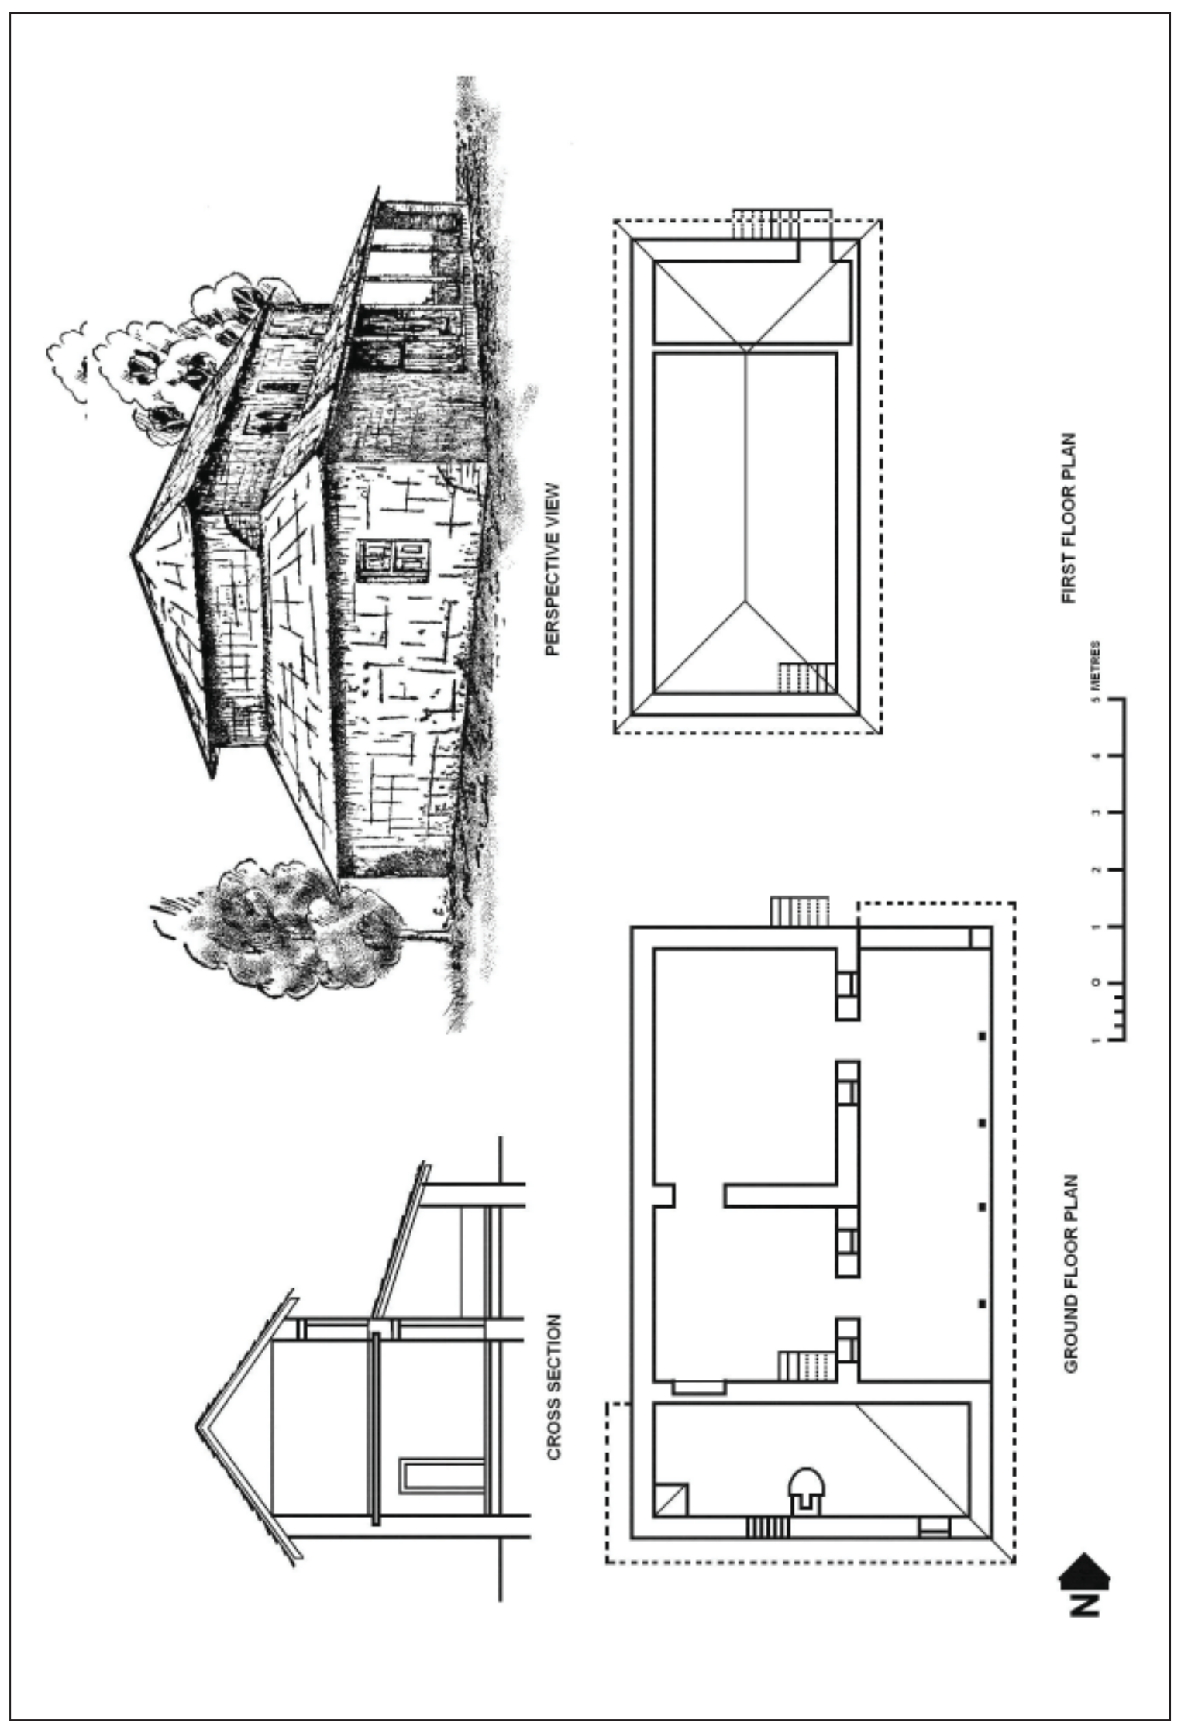
\includegraphics{images/chap02-01.jpg}
\caption{A typical house in village Hatali}\label{chap02-fig01}
\end{figure}

The rooms behind the veranda are of different sizes, varying accord ing to the taste and requirement of the owner. Gene rally, rooms measuring 3.04 x 3.65 m or 3.65 x 4.27 m are preferred. On one side of the veranda, an oblong kitchen-cum-dining space, running through the entire width of the house, is made. This kitchen is a multipurpose room, where, besides cooking and dining, utensils, grains and fuel wood are stored. Obviously, most of the indoor activity remains confined to the kitchen. Therefore, to make it commodious, the maximum number of niches and recesses of all shapes and sizes are made in the kitchen walls, which serve as cupboards to keep all sorts of household articles and wares. A hearth (\textit{chullah}) is constructed in the centre of the longer wall so that the family members can squat around it comfortably. No chimney is provided for smoke to escape. Only a fraction of it escapes from the door and the rest keeps on whirling in the interior, blackening the walls and ceiling. Traditionally, the hearth must always be kept alive with a smouldering fire. Extinguishing the fire in the hearth is considered a bad omen. A square spot paved with slates is provided in one corner of the kitchen to serve as a sink (chala) for washing utensils. The women also use this chala for bathing. The floor of the kitchen is kept slightly raised from the usual plinth level of the house to ensure the sanctity of the cooking and the dining area. Shoes are hence taboo in the house. The height of the room on the ground floor varies from 2.50 m to 3 m.

Another floor is raised over the main rooms only, leaving the kitchen and the front veranda single storeyed. The height of the first floor is restricted to between 2 m to 2.50 m. A house of more than two storeys is rare, and so are the single storayed houses uncommon in this region.

The possible reasons for preferring two storeyed houses may be functional as well as aesthetic. Since the rate of precipitation in the Jammu-Kangra region is very high, rooms on the ground floor may be unsafe due to excessive humidity and dampness, while the rooms on the first floor remain airy and safe, especially for sleeping during the summer and rainy seasons. Further, while a single storeyed house may look sunken and submerged among the thick groves of fruit trees and bamboo, and the three storeyed structures may not only be in disharmony with the surroundings, but may also be undesirable when there is ample scope for horizontal expansion.

The roofing style in Jammu-Kangra area is typical of the area and very beautiful. This style of roofing may not be found elsewhere in the western Himalayan region. The rooms on the first floor are covered with a high-pitched hipped roof covered with fine slates and the single-storeyed portion, which includes the fronting veranda and kitchen, is covered with the lean-to roofing covered with slate. To support the lean-to roof over the veranda, wooden posts are provided on the edge of the veranda at required spacing. These posts are sometimes placed on the well-shaped corbel stones (\textit{kursi}). Good quality slates are conveniently available in this region from the quarries on the slopes of Dhauladhar, and people use these liberally. The house with this type of roofing has the pleasant look of a chalet-type cottage, which blends harmoniously with the surroundings. However, in the lower part of this region, tiles are also seen in some traditional houses. Possibly, the cartage of slates from the quarries on the Dhauladhar range to far off places in the lowland country was expensive, therefore, the local \textit{kumhar} (potter) used to prepare baked tiles for their clients. However, no such tiles are manufactured now.

Good quality fine-grained sandstone is amply available in the entire Jammu-Kangra region and people have been using it extensively in residential houses and sacred and other secular buildings. Despite the superior quality of structural stone, people generally use it only for the foundation and ground floor, but those who can afford may use stone (or burnt bricks) for the first floor also. However, people generally prefer sunbaked mud bricks for the upper floors for economic reasons.

Whenever one proposes to construct a house, the family Brahman or \textit{chela} (oracle of the local deity) is consulted for selecting a propitious site. He approves the site by divination and it is earmarked by tying a red-dyed raw cotton thread. Some sweets are also be distributed on that occasion. On the appointed day, the foundation trench is excavated about a metre deep. The trench is then profusely watered and left exposed for a few days. It is then vigorously rammed to optimum compaction with \textit{durmat} (an improvised wooden or stone mallet), and then hand-packed with boulders to about half a metre thickness and properly rammed, plugging all gaps and voids with the binding material, earth, sand, grit, and so on. Over such a base, the random rubble stone masonry is laid in courses. People mostly use mud or lime mortar. Normally, no offset is provided in the foundation until the ground level, but one is provided at that level so that the width of the wall remains about 60 cm, which is reduced further at the plinth level to about 45 cm. The height of the plinth varies from place to place. While the height of the plinth is restricted to 22 cm and 30 cm in the rocky, uneven and well-drained locality on the slopes of Dhauladhar, it may be as high as 45 cm to 75 cm in the lowland area, where the ground is flat and susceptible to capillary action of water.

As the wall reaches the plinth level, the location for the doors is earmarked. Placing the main doorframe involves a ritual, which the carpenter performs. He ties a small pouch of cloth containing \textit{dhaniya} (coriander seeds), \textit{supari} (betelnut) and \textit{kusumbha} to the horizontal member of the frame with a \textit{mauli} (auspicious dyed cotton thread). Upon reaching the desired height of the wall, window frames are placed in position. During this process, niches are also left at different spots as per requirement. No lintels or arches are provided over the openings or niches, but a thick and stout wooden board, known as \textit{saldar} or \textit{sardal}, is placed to serve that purpose. When the walls reach the height of the ground floor, wooden beams are spanned across the width of rooms at a specified spacing. On such occasions, ritual worship is also performed. Over those beams, floor joists are placed at about 30 cm from centre to centre. Over the joists, walls are further raised to the roof level of the first floor.

After the construction of the four walls is complete, it is time to lay the roof so that the structure is adequately protected to carry out internal works. The conventional trusses are unknown to the traditional artisans, but they have evolved a simple but ingenious contraption for laying the roof. That under structure is called \textit{kainchi} in the local parlance. A \textit{kainchi} is an arrangement of a pair of rafters, with or without a tie-beam, placed at specified intervals on the outer walls to form isosceles triangles. To keep these rafters firmly in position, a ridgepole (\textit{lada}) is fixed at the lap-jointed apex of these rafters. The entire structure is further strengthened by the hip rafters and purlins (\textit{kadiyan}). The placing of \textit{kainchi} in position is celebrated by ritual worship and offerings. On the purlins, slates are nailed from the gable-end upwards, allowing sufficient overlap so that the storm water does not enter inside. A lap of about 15 cm is allowed on the ridge to ensure safety against leakage. Sometimes, semi-circular baked earthen tiles are placed on the ridge to cover the slate joints. The local \textit{kumhar} make these tiles to order. Completion of roofing is a big occasion to celebrate. On that occasion, the \textit{thawin} (carpenter) sits on the ridge, taking some flowers, rice and \textit{droob} (Sanskrit: \textit{doob}, shoots of green grass) in his hands, and pours water from a pot on the roof. He does not come down unless some reasonable offering is made to him. Such offerings include clothes and cash.

After completing the external operations, the internal works are taken up. These start with the laying of wooden planks for the flooring, but those who cannot afford wooden planks, use bamboo, reed or even dry twigs and bushes for the purpose. Over that base, mud flooring is provided. To prepare mud for that purpose, well-kneaded clay, blended with the binding material – rice husk or chopped chaff – is allowed to mature and season for a few days. It is then made into gara (mud mortar) and spread evenly over the base. When the surface is semi-dry, a floating coat of cow-dung is smeared over it to plug the cracks. When the coat is still moist, burnishing with the smooth pebbles (\textit{ghotani}) is done. The floor is then allowed to dry. Usually, a similar process is repeated for making the floor of the ground floor, but the base is made with boulders and grouted grits. Sometimes, people lay flagstones or shingles for that purpose. In that case, mud flooring is obviated, but cow-dung coating is mandatory to plug gaps in the paving. While laying the floor for the upper storey, a recess is left in one corner for the trapdoor, which provides access to the first floor from the ground floor through a portable wooden stepladder. However, an external stepladder or regular staircase is also provided.

Normally, windows are avoided on the back walls of the house, but are provided on the sidewall and in the front. These may be with or without shutters, but are mostly provided with iron gratings. Traditionally, no iron hinges were used to fix shutters, but those were held in position by the pivots. Such shutters produce a creaking sound when opened or shut.

For finishing, the external and internal surfaces of the walls are very neatly mud-plastered. For this purpose, clay and binding material are mixed together and well kneaded. The mixture is then allowed to mature for several days. It is then again kneaded into \textit{gara}. That medium is tightly and closely applied to the surface and finished by hand to ensure a smooth surface. When semidry, a floating coat of clay and cow-dung solution is applied to seal the cracks. When the surface is dry, white washing and colour washing is done. For this purpose, people use white earth or \textit{golu}, and ochre or \textit{losti}, for white or colour washing. Colour washing is done up to a height of about 70 cm from the ground level. A strip of \textit{losti} is also provided all around on the outer face under the gable, but the rest of the outer surface of the wall is whitewashed. All this painting work is normally done by the women of the household themselves. The women of Jammu-Kangra area are very keen on wall decoration, and to add an aesthetic touch to the house, they painstakingly make interesting linear drawings, depicting numerous floral, faunal and figurative devices. In fact, decorating houses with such drawings is regarded auspicious for the household. The door and window openings are particularly decorated to usher in prosperity and fecundity to the house. On various festive occasions, such as Diwali, weddings, and so on, even the front door and front courtyard is profusely decorated with various earthen colours (Figures 2.2, 2.3 and 2.4). Paints and glasses have traditionally been unknown, but of late, these are becoming common.

\begin{figure}[!htbp]
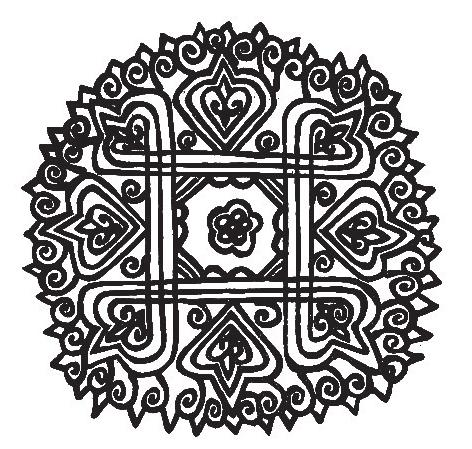
\includegraphics[scale=.4]{images/chap02-02.jpg}
\caption{An auspicious floor design for Diwali festival}\label{chap02-fig02}
\end{figure}


\begin{figure}[!htbp]
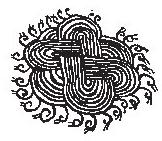
\includegraphics[scale=1.21]{images/chap02-03.jpg}
\caption{A floor decorative design for ceremonial occasions}\label{chap02-fig03}
\end{figure}


\begin{figure}[!htbp]
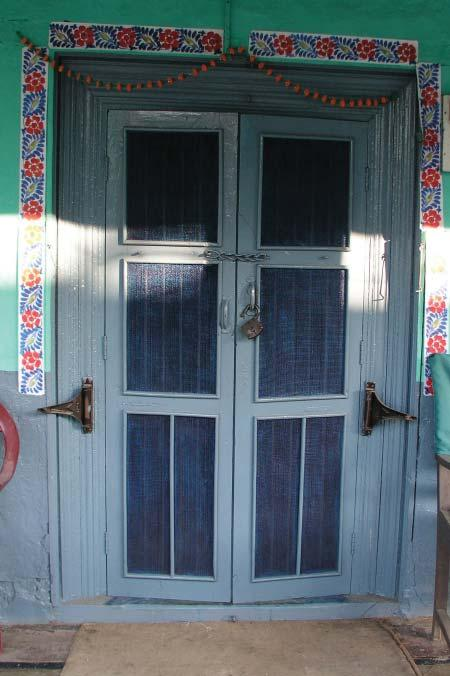
\includegraphics[scale=.3]{images/chap02-04.jpg}
\caption{Traditionally decorated main door of a house}\label{chap02-fig04}
\end{figure}


\subsection*{Lowland House in a Temperate Setting}

Chalet-type cottages are preferred in the upland country on the slopes of Dhauladhar, where the soil strata is rocky and well-drained, and structural timber is conveniently available. In the undulating lowland area, where wide stretches of the fertile \textit{kyar} (wet paddy fields) exist and the area is under green forest cover, chalet-type houses are fewer. Under the obtaining humid and damp environment, the use of wood has been considerably minimised. Here, the houses are laid out in a quadrangular form, have the stone masonry plinth as high as 45 cm to 75 cm. Even the four walls of the ground floor may be built of rubble stones. However, sundried bricks may be used on the first floor. In any case, the choice of material depends on its affordability. The mud-based walls can be raised without skilled labour. These can also be maintained by household women in a routine manner, but these are certainly not long lasting. On the other hand, the construction and maintenance of stone or burnt brick walls (Figure 2.5) which are long lasting, need skilled masons.

\begin{figure}[!htbp]
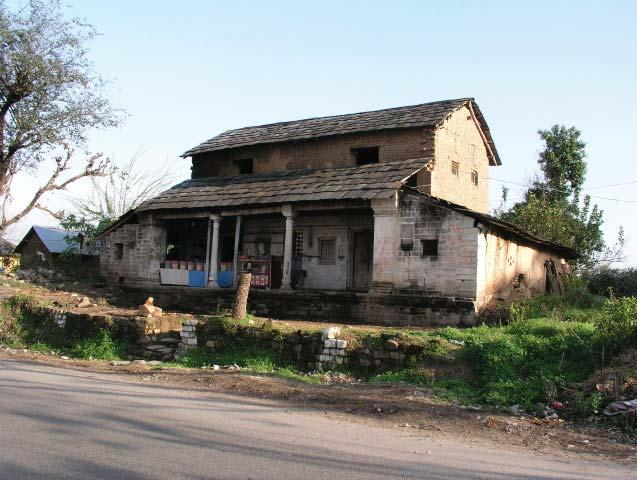
\includegraphics[scale=.35]{images/chap02-05.jpg}
\caption{A lowland house made of mud-bricks and stone}\label{chap02-fig05}
\end{figure}

\newpage

While the material of construction and the arrangement of rooms remain almost the same as in the highland houses, the interior here is more roomy and airy, with more windows and larger windows. The verandas of these lowland houses are deeper. Further, the roofing arrangement is considerably altered to minimise the use of wood, and so the wooden posts of the veranda are replaced by masonry pillars. Instead of the hipped-roof, gabled roofing is preferred in this lowland area, for such a roof requires less wood and does not let the snow accumulate, thus preventing extra load on the structure. However, care is taken to project the roof at least 70 cm to 80 cm from the outer faces of walls on all sides to protect them from slant showers.

The roof over the veranda is the lean-to type, and made in a casual manner, giving an impression that the veranda does not form an integral part of the original planning, but is a later addition. In fact, up to the plinth level, the walls of rooms and the fronting veranda are constructed simultaneously but after that only the walls of the rooms are taken up to a double storey height. The work on the veranda is withheld until the double storey structure, including finishing, and so on, is complete. The reason may be that the filling of the veranda floor should become thoroughly compacted by the movement of workers and rainwater, while the rest of the house becomes habitable. After the veranda has been properly weathered, it is finished. Heavy stone or brick masonry pillars are erected on the edges at the required spacing (Figure 2.6).

\begin{figure}[!htbp]
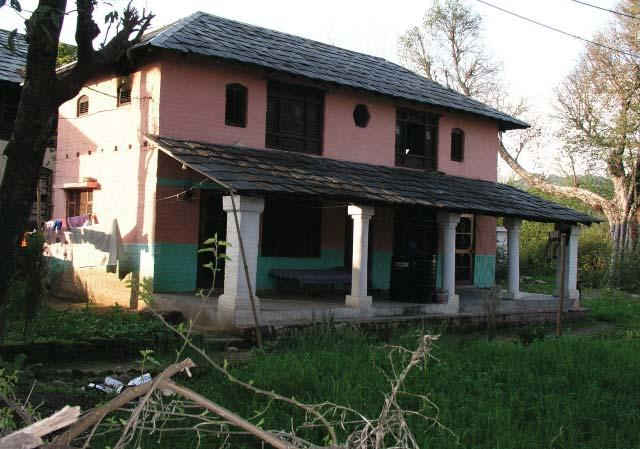
\includegraphics[scale=.35]{images/chap02-06.jpg}
\caption{A lowland stone-built house of the Jammu-Kangra region}\label{chap02-fig06}
\end{figure}

These pillars can be round or square in cross section, depending upon the choice of the owner. Over it, a wooden breastsummer is placed. Over it, the roofing joists are spanned, with their upper ends inserted at a higher level in the wall so that a regular lean-to slope is attained. Mostly corrugated galvanised iron (CGI) sheet roofing is provided over the veranda, while fine slate roofing is a common practice for the main building. In certain cases, even a thatched roof may be seen over the veranda.

The lowland Jammu-Kangra area is generally humid, with numerous irrigation channels and streams flowing around, keeping the sandy loam soil damp, thereby providing the most congenial conditions for termites and other insects to thrive, which are most injurious to wood. Therefore, extreme care is taken to avoid contact of wood with the ground. For that purpose, not only is the plinth kept higher, but also the thick stone slabs, large enough to cover the width of the wall, are placed under the door and window openings so that the sill is further raised. Thus, one has to step up from the veranda to the sill and step down into the room. Thick flagstones are also placed at the plinth level on the outer edge of the veranda.


\subsection*{Highland Double Storey House in a Temperate Setting}

Sprawling over the gentle and fertile meadows on the slopes of Dhauladhar, Chauntra is one of the most picturesque villages of the Jammu-Kangra area, in the Mandi district. The scenic charms of this village increase manifold with the snow-capped crest of the Dhauladhar forming a magnificent backdrop; tea-gardens all around and the toy-train chugging on the Pathankot-Jogindarnagar narrow-gauge railway line. The bracing mountain-air wafting through the pine, the rhododendron and ban forests around impart a salubrious ambience to this village. The climate of Chauntra remains bracing throughout the year. Even in summer, the temperature does not exceed $30^{\circ}$C. Pleasantly enough, a slight increase in temperature is invariably followed by gathering clouds and a soothing downpour. Thus, the climate remains bracing even during summers; winters are sunny and moderate, though the village occasionally experiences mild snowy conditions.

The village is located on the thick layer of porous sandy-loam overburden over the rocky substrata, with the gentle slopes to the perennial rills -- Bajgar Khad and Makkar Nal -- on the sides. Thus, the place is secure, hygienic and comfortable to live in. These streams provide uninterrupted water supply for drinking and irrigation purposes. The village is spread in three well-spaced clusters -- the Nichala Chauntra, which was the original and proper village. The railway line also passes through this cluster. Later, with the establishment of a tea-factory, habitation also developed around it. Further, the village also expanded towards the Mandi-Pathankot highway. People built houses and shops along the highway. Besides, a school building also came up there. Thus, a separate cluster of houses was formed, which is known as Uparala Chauntra. Since ample open land is available on all sides, the village has expanded horizontally on all sides, with houses well spaced out.

Chauntra is a multi-community village, inhabited by the Brahmans, business, agrarian and professional communities. Among these communities, the Sood business community is economically better off and the professional communities constitute the lower strata of the village social setup. However, agriculture is the mainstay of the people. Although the layout and architectural pattern of the houses of this village is broadly not much different from the rest of the Jammu-Kangra region, yet the moderate climatic conditions, agrarian livelihood of the people and their economic status are well reflected in the planning of the village houses. Keeping in view these considerations, one comes across different types of layout patterns here. Thus, most of the houses belonging to the majority peasantry are built on the linear layout. Then, there are the houses with ‘L’ or ‘U’ type plan. These belong to the better-off Brahmans, agrarian and professional households. However, there are a few houses with quadratic layout, mostly owned by the moneyed Soods. Such houses are known as the chowki. One of the wings of a chowki, facing the road or street may be used as a shop, but that is not a common practice. As a rule, all houses in the village are double storeyed, and this holds good for the houses in other villages nearby. While most of the ‘L’ shaped and linear houses have no covered veranda, all the houses with square (chowki-type) or ‘U’ type layouts have internal covered verandas on both the floors. The covered veranda on the ground floor is known as the otta, and the one on the first floor is called paura. Every house has a spacious and well-kept courtyard (angan). Kitchen gardens and agricultural fields surround most of the houses in the villages. It may be appropriate to discuss the aforementioned types of layouts before we take up the construction techniques.


\subsection*{\textit{The Linear House}}

In the houses with a linear layout, there are normally two rectangular rooms on the ground floor (Figure 2.7). These rooms on the ground floor are known as the \textit{obara}. On the first floor, usually a large oblong room is made, but there also could be two rooms corresponding to the arrangement on the ground floor, depending upon the resources and requirement of the family. These rooms are generally very spacious and airy, on the average measuring about between 3.70 x 4.50 m and 4.50 x 6.00 m. The rooms on the ground floor are entered through the open fronting veranda, which, in fact, is an open platform at the plinth level. Each room has a separate door (\textit{bheet}) and a window (\textit{dwari}). Usually, the rooms are interconnected with an internal door. Sometimes, in place of a window, a round or square grated opening is provided. From one of the obara, a single flight stepladder with a trapdoor is provided to the room on the first floor. This \textit{obara} is a multipurpose room, serving as a kitchen and living room and used for sleeping during the night. In order to make space for the utensils and other kitchen items, niches and recesses (\textit{lakore}) are made in the walls. The other \textit{obara} is used for sleeping. The accommodation on the first floor is usually used for storing grains and other household items. For most part of the year, the family is confined to the accommodation on the ground floor. However, living on the ground floor during the rainy season is considered injurious to health. Therefore, people shift to the upper floor during that period, especially for sleeping during the night. The linear house generally has a gabled roof (\textit{dhalwan chat}), covered with slates, but thatched roof (\textit{chhanan}) is also common on the linear houses. However, some hip-roofed houses are also found. Care is taken to project the roof sufficiently beyond the walls to protect them from direct rains. Such a projection is locally known as \textit{chhapraur} or \textit{chhaprauti}.

\begin{figure}[!htbp]
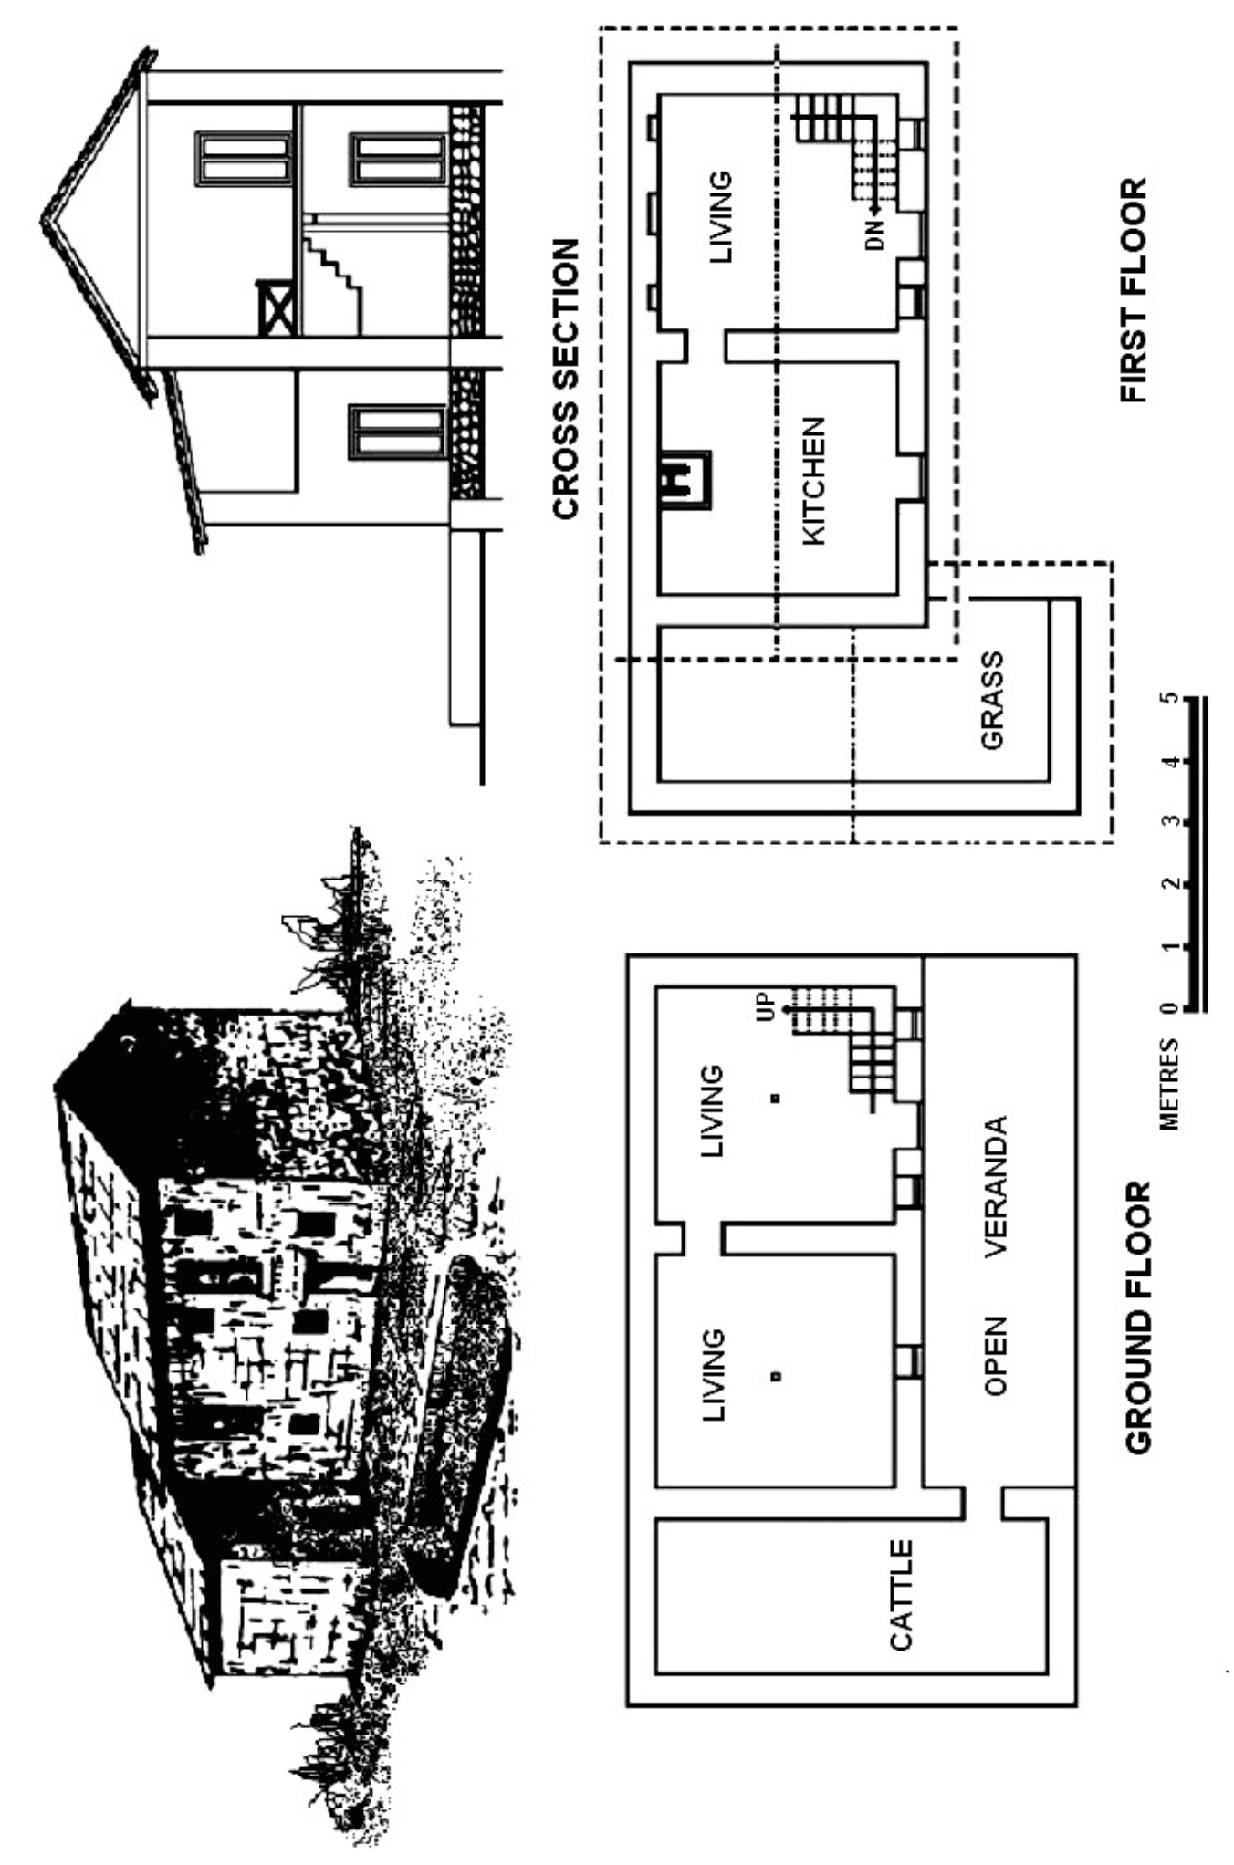
\includegraphics[scale=.85]{images/chap02-07.jpg}
\caption{A highland double storey house at Chauntra}\label{chap02-fig07}
\end{figure}

In front of the house, a sunken and paved rectangular courtyard (\textit{khwala}) is maintained. It is always kept well-trimmed and neat. Not only are the outdoor household chores performed here, but also agrarian operations, like thrashing, cleaning, winnowing of grains, and so on, are done there. A small thatch-roofed hut is made separately at a close distance for the cattle.


\subsection*{\textit{The ‘L’- and ‘U’- shaped Houses}}

The ‘L’ shaped house is only an improvement over the house with a linear layout. In fact, the ‘L’-shaped house is raised on a linear layout up to the plinth level, but beyond that, the superstructure is raised to a double storey height in an ‘L’-shape. In addition to what has been noted above with reference to the linear house-type, an oblong room is added on one side of the house to form an ‘L’-shaped superstructure. This additional room runs through the entire width of the building (including the open veranda) on one side. This additional oblong room serves as the byre for tethering milch cattle. The room over the byre serves as a lumber-room for storing fodder, agricultural implements, and so on. No door to that lumber-room is provided, but a part of this room towards the platform on the ground floor is kept open. To enter the lumber-room, a portable bamboo or wooden ladder is positioned on the platform, so that one may climb into it.

\newpage

There are a few houses with the regular ‘L’-shaped layout at Chauntra and the villages around. Such houses have covered verandas on both the floors, from which the rooms behind are accessed through the doors or bheet. Access to the first floor is provided through a regular single flight or a doglegged wooden staircase (\textit{sangah}) from one corner of the veranda. In such regular ‘L’-shaped houses, there is no provision for the byre, and the cattle are tethered in a separate shed, away from the house. The ‘U’-type house is an improvement over the ‘L’-type as another wing is added to the ‘L’-type layout to form a ‘U’-type layout. With the exception of a few ‘U’-type traditional buildings, such houses are rare not only in this area, but in the entire Himalayan region. A typical example of the ‘U’-type edifice may be the ancient castle palace at Kotkhai in the interiors of Shimla Hills (Handa 1997: 116-118).


\subsection*{\textit{The Chowki-type House}}

A house built on a quadratic (rarely rectangular) layout, enclosing a spacious and open paved courtyard (\textit{angan}), is known as the \textit{chowki}. The \textit{angan} is a central and an important part of a \textit{chowki}, where all the family functions are performed. In the centre of a chowki, an elevated ornamental vase is made, in which basil plants (tulsi) are grown. Adjoining the tulsi vase, a small one-piece tri-stepped votive stone, known as the mandala, is installed. On the top surface of the mandala, a stylised lotus device is carved to form a magic diagram (Sanskrit term – mandala). This tri-stepped votive stone may be a popular rendition of the classical Buddhist stupa. The married women of the house are required to perform pooja and offer water to the tulsi and mandala every morning.

The chowki-type house essentially is a four-winged double storeyed structure, with all the four wings having a spacious running veranda on both the floors, facing inwards. The veranda on the ground floor is locally known as the otta, and the one on the first floor, known as the paura. These verandas remain alive with activity not because all the rooms on both the floors have entrance from the verandas, but most of the waking hours of the family are also spent there. On the outer edges (bheen or bheend) of the veranda on the ground floor (otta), artistically chiselled and carved pedestal stones (kursi), chiselled to form stylised pots, are placed at the required spacing. On those kursi, wooden posts (thamb) are erected to support the floor joists (karian) and floor planks (phare) of the upper storey. On the outer edges of the running veranda on the first floor (paura), an ornamental wooden railing (binag) is provided between the wooden posts. These posts provide the support for the lean-to roof over the veranda. Depending upon the size of the chowki, it may have one or more fixed straight flight or dog-legged staircases on the angles.

Entry to the chowki is provided through a gap left in one of the wings. It is called praur. Such passage opens into the central courtyard, and one is required to climb up to the veranda to enter into the rooms. Sometimes, an anteroom is provided on the ground floor that has its main entrance from the street. That entrance-room is known as the wan. The wan is normally enclosed on three sides, but without any wall on the fourth side that opens into the veranda. One may step out onto the veranda from that open side to go inside the building.

The chowki-type house is an elaborate building, with a number of rooms on each wing of both the floors. The size of the rooms on both the floors is identical. While the arrangement of doors is similar on both the floors, there could be variation in the arrangement of windows and niches. All the rooms of a chowki have separate doors to enter through the fronting veranda on both the floors. These may or may not be interconnected from inside. The size of a chowki and the interesting woodwork and stonework in it, which in some cases is very artistic and profuse, may speak volumes about the economic affluence and prosperity of the person, who built it to accommodate a large and extended or joint family during the pre-Independence period. However, with the joint family system now almost obsolete, some of the rooms in such a large mansion may be lying vacant and unused for decades, or being used as lumber-rooms. In many cases, with the division of a family, the rooms of a chowki have been divided among the stakeholders. That has disturbed the original arrangement of a chowki under the obtaining situation. In certain cases, even structural changes have been made to meet the requirement of the family under the altered conditions, thus distorting the traditional character of the architecture.

The chowki-type houses in Chauntra, as elsewhere in the Jammu-Kangra region, belong to the prosperous Sood, Mahajan, Gupta and Khatri, all belonging to the business community. In the mid-Himalayan interiors, even the Brahmans have chowki-type houses at many places, as in the Karsog area of Mandi district. Traditionally, these communities had been landowners, who never cultivated land, but leased it out to the cultivators on a crop-sharing basis. Thus, in their chowki, one may find granaries and large wooden containers (kothad) and bamboo silos (pedu) -- one example of which is shown in Figure 2.8 -- on the ground floor, but no lumber -room or byre for cattle. Some of the households maintain milch cattle, but the sheds for tethering them are built separately, away from the chowki.

\begin{figure}[!htbp]
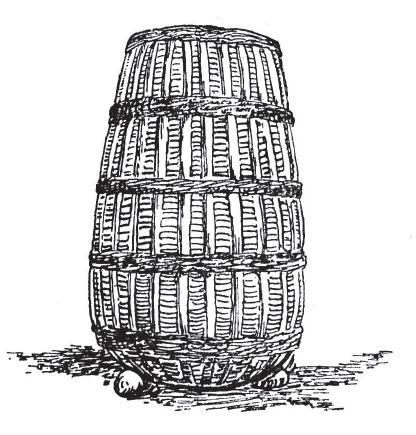
\includegraphics[scale=.42]{images/chap02-08.jpg}
\caption{A pedu for storing grains}\label{chap02-fig08}
\end{figure}

In case there is no room in one of the wings of a chowki, that wing is known as the naswal. In the chowki, the kitchen (rasoi) is always kept on the upper floor in a corner. While the family members may take their food in the spacious kitchen itself, a formal guest is served in the paura or the living room (baithak). When a separate room is earmarked in a chowki for keeping water pots, that room is known as the jalaihar. In one corner of the paura, a paved enclosure is made for bathing and cleaning of utensils. Customarily, no toilet is provided in the chowki, but a dry latrine (swari or jajaru) is improvised, separate and away from the chowki, for the female members of the household. The males are supposed to ease themselves in the open. The chowki is always provided with the slate- covered gabled roof over the rooms and the lean-to roof over the verandas.


\subsection*{\textit{Materials and Method of Construction}}

Once a proper site near the fields, where water is avail able, has been selected, the foundation (niyun) trench is excavated after due rituals. Since the soil strata in the locality are sandy-loams and porous, the foundation has to be dug to a depth of one metre or more until hard strata are found. The width of the foundation is kept between 60 cm and 75 cm. The bed of the foundation is watered and rammed with a heavy wooden or iron mallet or durmat to ensure thorough compaction and evenness. That is followed by the hand filling (bharti) of foundation with coarse boulders to a thickness of about 20 cm to 25 cm. The filling is thoroughly rammed, watered and the voids are filled with sand and grit. People prefer to leave the foundation exposed to the summer rains so that it is properly settled and weathered, after which it is further rammed.

On an auspicious day, a ceremony is performed to lay the foundation stone after which the work progresses further. The thickness of the wall up to the ground or plinth level is normally kept the same as the width of the foundation. However, of late people are opting for the offsets in foundation for economy. Ordinarily, dry masonry is used and the walls are raised up to the plinth level, that is, to a height of about 45 cm. At that stage, the floor area between the walls is thoroughly soaked with water and filled with the soling material, such as grit, flints, brickbats, and so on. It is then thoroughly rammed so that the filling is level with the walls. The doorframes (dwar-shakha) are then erected on the plinth wherever necessary. Placing of the dwar-shakha is followed by a ritual worship, during which a red mauli (raw cotton thread) is tied to it.

After the doorframes have been fixed in position, the masonry work is continued further. Similarly, window frames (chaukhat) are also placed in position when the walls reach the window level. A single window is considered sufficient for each room. As the work of raising walls continues, niches and recesses are left at proper places. Around Chauntra, good structural stone is not available in the locality. People mostly use the local mica-laden white hard granular stone for con struction of walls up to the plinth and for the outer walls of the ground floor. In situ moulded, sundried mud bricks of 25 x 12 x 6 cm size are used for the inner walls on both the floors and the outer walls of the first floor. The thickness of outer walls is normally 45 cm, but the internal walls on both the floors are usually made of a single brick thickness.

When the construction of walls is complete up to the first floor level, a wooden beam (shaiteer) is placed across each room on the shorter span, over which wooden joists or karian are spanned. Where bamboo is available, people use it for karian to ecnomise, for structural timber is not easily available and is very expensive. The height of the rooms on the ground floor of the houses in Chauntra and other neighbouring villages is about 2.50 m, for the first floor, it is about 2.25 m.

After the basic woodwork of the first floor is complete, the walls are raised further up to the roof level in a similar manner as for the ground floor. In the process, doorframes (dwar-shakha) and window frames (chaukhat) are placed in position and the niches and recesses, where required, are provided.

After the walls have been raised up to the roof level, work for roofing is initiated. For the gable roofing, the extreme sidewalls are raised further to form structural gables to support the ridgepole (lada). While the houses with linear, ‘L’-type and ‘U’-type layouts may be provided with the gable or hipped roofing, the roof over the chowki-type houses has to be necessarily gabled, with hips and valleys on the corners. The local traditional baddhi prepare roofing infrastructure by positioning rafters (bala) on the lada and the side walls, duly fixed in position by the tie beams, at the required spacing. Those contraptions are called kainchi. The ends of the bala project sufficiently from the outer edges of the walls to form projected gable-ends (chhapraur or chhaprauti) on the sides. Over the kainchi, purlins (karian) are placed at the spacing that varies depending upon the roofing material, which may be slate or thatch (chhanan). Wood is mostly used for the roofing substructure, but some people use bamboo for economic reasons. Normally, the ceiling is avoided in most of the houses for economic reasons, but in the chowki type houses, the ceiling may normally be found in a few rooms. The space formed between the ceiling and the roofing is known as the tarha, the loft.

The work for finishing and internal fittings is then taken up. The floor of the ground floor is generally made by a thick layer of the gara (thick mud mortar) over the soling layer of grits, flints, and so on. Over the semidry gara, a thin layer of cow dung is applied. In the first floor, mud flooring is provided over the phare or wooden planks or the bamboo scantlings. Sometimes, no mud flooring is provided over the phare, and these are kept exposed. The walls are also plastered (maidagi) from both sides with gara and finished with a floating coat of cow-dung solution. When the maidagi is dry, the walls are whitewashed with the local white earth (makol) or colour washed with losti.


\subsection*{Housing Pattern in the Subtropical Arid Environment}

There are certain pockets in this region, where the soil is composed of the rugged conglomerate strata. Such strata can hardly retain water to sustain cognisable vegetation except the sparse subtropical thorny and semi-desert vegetation and the local variety of bamboo and grass, such as bhabhar or bagar, lamb (Heteropogon contortus Beame.), and so on. Structural wood is scarce in such localities. Therefore, people mostly use bamboo (except for the door and windows) in place of wood for their residential houses in such areas. In fact, bamboo is a staple material for flooring and roofing purposes.

Most of the residential houses in the villages on the Sikandra Range, which roughly separates Mandi, Hamirpur and Bilaspur districts of Himachal Pradesh, fall in such arid and hot geo-climatic region. Although for construction of walls, good quality stone is available in this area, people use it only for foundation, and occasionally for the ground floor also. For the first floor walls, normally sundried bricks are used or rammed earth walls, locally known as the matkanda, are made (Figure 2.9).

Kot is one of such villages of the Jammu-Kangra region, where subtropical arid environmental condition prevails for most part of the year. It is a medium-sized multi-caste martial village of the Sarkaghat tehsil (Mandi district). The village is sprawled over the narrow and rugged terraces of a sub-range of the Sikandara Range (Sikandar Dhar), reaching down to the Bakkar Khad that forms the border between Mandi and Hamirpur district. This seasonal stream is notorious for its treacherous behaviour, as a popular saying goes:

\begin{figure}[!htbp]
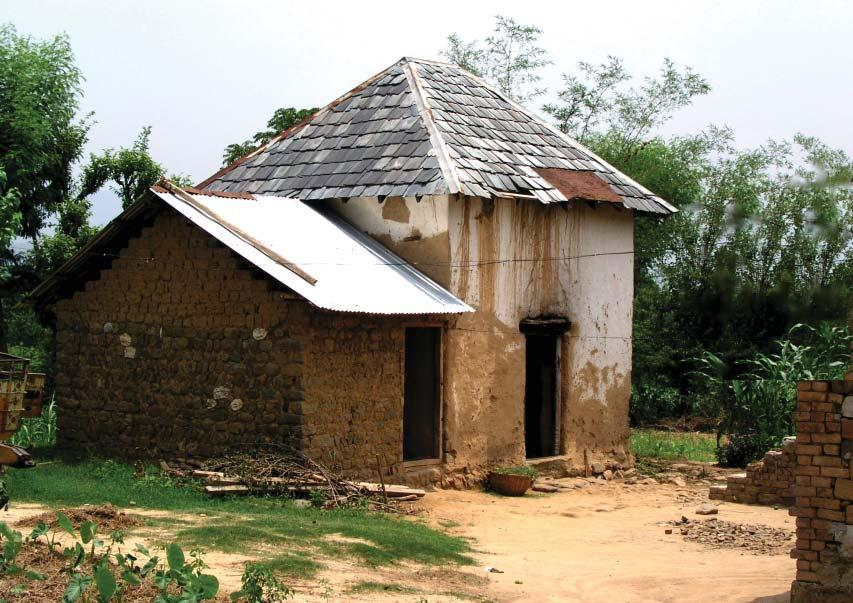
\includegraphics[scale=.3]{images/chap02-09.jpg}
\caption{A typical house in village Kot in the subtropical arid environment}\label{chap02-fig09}
\end{figure}

\begin{myquote}
\textit{‘Bakar khad sab khadan di ranee,} \\\textit{Hiyunda dhoop na taundi pani,} \\\textit{Barasatee jan kyian bachanee.’}
\end{myquote}

\newpage

Translated, this saying means:

\begin{myquote}
‘Bakar stream is the queen of all streams,\\ Winters here are sunless, summers dry,\\ The pluvial spells are treacherous well nigh.’
\end{myquote}

In fact, this seasonal stream remains completely dry for most part of the year, but during the rainy season, it is unpredictable and at times, not fordable. The rugged landscape of the area is devoid of any type of natural vegetation. People have planted trees on the edges of their terraced fields and around the village to ensure the supply of fuel and fodder for their livestock. The village has scat tered habitation, roughly forming three irregular clusters on three separate hillocks. Two of them, belonging to the higher castes, are in close proximity, and the third one is at a small distance. However, all those clusters are interconnected by several foot paths. Customarily, the houses of the higher caste families are the double storeyed and slate-roofed structures, but the ones belonging to the lower castes are generally single storeyed, thatched roofed dwellings. However, the class distinction no longer holds good and such distinction is now based more on economic considerations. One may find even the double storeyed houses covered with thatched roof (kareen) and single storeyed dwellings with fine slate (chakka) roofs, belonging to any community.

Thus, in this village, two types of houses may be found. There are a few single storeyed houses, but most are double storeyed. Again, very few houses have thatched roofs; most of them are covered with fine slates. Very few houses also have CGI sheet (teen), roofing. People prefer slate roofing, for these provide better insulation against the scorching heat of summer and the chill of winter, while the CGI sheet roofing gives much protection against either. Further, the slate is a permanent and maintenance- free roof-covering material, while CGI sheets are prone to weathering and rusting; however, thatched roofing is a potential fire hazard. For these reasons, the people of this subtropical and arid area, including Bilaspur district and part of Solan district, prefer double storeyed houses covered with slate roofs (Figure 2.10).

\begin{figure}[!htbp]
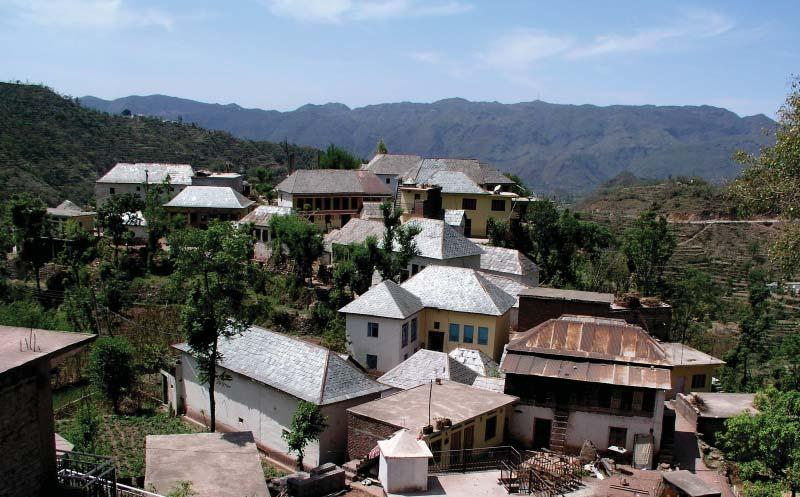
\includegraphics[scale=.35]{images/chap02-10.jpg}
\caption{A clustered arrangement of houses in the subtropical setting}\label{chap02-fig10}
\end{figure}

These houses are laid out in the well-trimmed quadrangular or ‘L – shaped’ form and are neatly built, with a stone or slate paved spacious angan, which generally is oriented towards the northern aspect (depending upon the local site condition), so that it may remain in shade for most of the summer months. People of this area spend most of their daytime hours in this courtyard, and some even prefer sleeping outdoor in the angan during the summer nights, when there is a cool breeze in the courtyard. In order to protect the interior from exposure to the sun, no windows are provided on the southern aspect, but ample openings are provided on the opposite side.

The houses in this subtropical and arid environment are roomy and well-ventilated, but normally without the fronting veranda. Even when a veranda is provided, it is never open, but enclosed, with only small windows and an entrance door. While the house is without a veranda, all the rooms, at least on the first floor, have to be interconnected.

Internal access to the first floor may be provided from one of the rooms on the ground floor through a stepladder or sangah, and a trapdoor. However, such an internal arrangement is uncommon. People prefer external access from the courtyard to the first floor. For that purpose, a solid masonry straight-flight staircase is made. Under the staircase, a spacious elevated niche is made for safely keeping the water pitchers. Since water is a precious commodity in this arid tract, not a drop is allowed to be wasted. People procure water from their specified borrow pits, locally known as the khati.

These khati have been the only traditional source of water for the people of Kot village, and many other villages in this arid belt. A khati is made by digging a deep and inwards slanting pit in the conglomerate strata on the hill slope. The drops percolated through the conglomerate strata on the side and roof of the pit gather to form a pool at the farther and deeper end of the pit. Thus, fresh and clean water is collected. In order to protect the water from pilferage, the mouth of the khati is provided with a sturdy battened and braced bamboo door and locking arrangement. Each family of Kot village has its own khati. In the event of marriage or other social functions in a family, water is borrowed from the khati of other households, which the family is customarily supposed to return to those households on similar occasions. Now, when piped tap water has been provided by the government, people prefer drinking water from the khati, for they consider it better than the piped supply.

In a double storeyed house, the rooms on the ground floor (aour) are normally used for kitchen (rasoi), storage (ohari), living (baithak), and so on. The room for the kitchen is positioned closer to the niche under the staircase, where water pitchers are kept. On one corner of the kitchen, a slate paved sink (chala) is made for cleaning utensils. Since a watermill (gharat) is rare in this arid tract, one may find a pair of grinding wheels (ghultoo) installed in one corner of the kitchen in every traditional house. For washing clothes and bathing, an enclosure is always improvised on one corner of the angan. The corner room on the ground floor of a double storeyed house is normally used as cattle shed (gohar). In case of single storeyed houses, a thatched cattle shed is made at a distance from the house.

For constructing a house, a site nearest to the fields is selected. Construction work is taken up after performing the usual religious rituals, after which the site is levelled and foundation trench (khali) is excavated about a metre deep. After proper ramming, it is hard-packed with boulders and grit, gathered from the bed of the Bakkar Khad. The walls of coursed or random rubble stone are raised up to the plinth level, that is, about 30 cm or 45 cm above ground level. Over the plinth, most of the walls are made either of rammed earth or of sundried bricks. The rammed earth wall is known as the bhittwali chinai or the matkanda. During the process of constructing bhittwali chinai, care is taken to leave openings at proper places to subsequently fix the frames for the doors (duar) and windows (taki). The sundried bricks made in this area are usually of 30 x 10 x 8 cm in size. In some instances, where good quality stone is easily available, houses, made of the random or coursed rubble stone masonry in mud mortar may also be seen. Of late, stone or brick masonry in cement mortar is becoming popular for building construction. The width of the wall is usually 45 cm.

In a double storeyed house (Figure 2.11), when the walls have reached the first floor level, the infrastructure for the first floor is laid. Since wood is scarce in the area, normally bamboo strips are closely spread over the wooden joists. Over that bamboo ‘planking’, about 5 cm thick layer of mud is spread. The construction of walls for the first storey is then carried out in the manner already described.

With rare exceptions, the roofs of houses in this area are of the hipped form: with slopes on all the four sides. These roofs are covered with fine quality slates. In some cases, thatched and CGI sheet roofs may also be seen. No slate quarry is available in this area, but the people import these slates from distant quarries on the slopes of Dhauladhar in Mandi and Kangra districts. The infrastructure for roofing is generally made of bamboo, with minimum use of scarce wood.

\begin{figure}[!htbp]
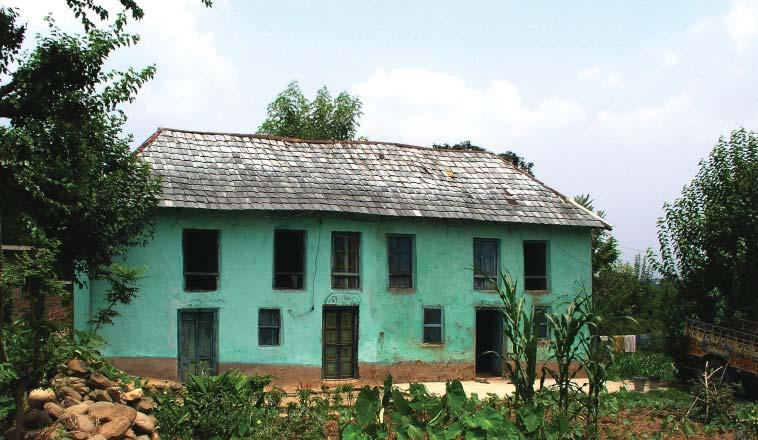
\includegraphics[scale=.36]{images/chap02-11.jpg}
\caption{A façade of a double storeyed house in the subtropical setting}\label{chap02-fig11}
\end{figure}

After the house is roofed, finishing work is taken up. The outer and inner surfaces of the walls are neatly plastered with mud. The womenfolk of this area are experts in plastering work. They not only ensure satin-smooth surfaces, but also execute interesting relief decoration on the matte earthen surface, depicting floral, faunal and figural motifs. Peacock is one of the most favourite motifs of such wall decoration. After plastering, the entire outer surface is treated with a fine coat of the locally available smoke-grey clay. This clay is very soft and sticky when wet, but becomes powdery when dry. Therefore, women mix rice starch (lugari or pitchh) with that clay to prepare a floating solution. Thin coats are repeatedly applied with grass-brushes (kutchi). The interior is either white washed or treated with a coat of smoke-grey earth.


\subsection*{Housing Pattern in the Doon Highlands}

The geo-climatic and biophysical scenario is different in the upland area east of the Satluj, in Solan and Sirmaur districts of Himachal Pradesh, which the author has defined as the Doon highlands. The villages in this hilly tract are usually located in a linear formation on different terraces along the contours, but where flatter locations nearer to the natural water sources are available, houses in clusters may also be found. Because the agricultural holdings of the villagers are generally located in a scattered manner, away from the habitations at various isolated places, many villagers have built their houses nearer to their fields on the rocky terraces, which normally are unfit for cultivation. Although the land in this tract is largely unsuitable for traditional agriculture, yet the people have been growing coarse grains, especially maize, and millets, with rain-fed irrigation. To protect their crops from wild animals, people build a singleroom shed on the strategic corner of their fields to keep watch over the crops. That improvisation is locally known as the doghari or dogari, that is, the second house. In fact, it is a farmhouse of sorts. One of the male adult members of the family lives in that doghari to keep watch over the crop. For the remaining period, that shed is used for keeping bullocks and dry cattle.

This hilly tract, abounding in the resinous cheer pine forests on the slopes, remains generally warm to hot and dry, with only moderate rain. It may snow occasionally on the higher reaches during the peak of winter, but the snow does not remain here for long; within an hour, it melts away. The overburden of stiff, dry and gritty red-ochre clay, deposited on the limestone base, is shallow and rocky in parts. This clay is very sticky and water-resistant. It does not allow water to percolate into the subsoil. Thus, the rainwater simply flows down through the seasonal storm channels and streams into the Sirsa in Nalagarh area and the Markanda and Bata rivers in the Kyarda Doon. Even the occasional layer of vegetable mould has in no way been able to improve the quality of this soil for agriculture, and it has been unsuitable even for traditional dry farming. Because of poor returns from agriculture, people have been seeking other vocations away from their homes for livelihood. Some households also subsist on dairy farming. For that purpose, they prefer buffaloes to cows. Mostly, people tether buffaloes in the open yard away from their houses. Sometimes, an open grass-roofed shed is made to keep the cattle during the cold winters.

Nevertheless, this sterile red-ochre clay has been good for building purposes, for this clay has good structural qualities. When wet, it is soft, sticky and pliable, thus, easy to handle, but when dry it become very hard, compact, and strong and has a very good bonding quality. At many places, good structural sandstone is also available in this area, which the locals use to build their houses. In this area, one may generally find single storeyed dwellings, built along the mountain slopes in a scattered manner in isolated settings, but a few double storeyed houses may also be found. In fact, the economic boom lately ushered in by the cultivation of non-traditional and off-season cash crops and vegetables has not only bound the people with their homes and fields, but also encouraged them to import new construction techniques and materials from outside to build their ‘modern’ houses. Therefore, no wonder that one may find somewhere a large and beautiful modern house set in this parched and rugged landscape.

For the study of a typical traditional residential house of this area, a house in village Ber-ki-Ser in the suburbs of Solan town, was selected. This village is inhabited by a heterogeneous community of people, which largely subsists on the mixed economy, in which agriculture plays only a supplementary role. Under such compulsions, extended or joint family system, as are found in the agrarian families, is almost missing here. People prefer a self-contained nuclear family system. This aspect is very strikingly reflected on the planning aspect of houses in this village. There is no open threshingyard around the house nor is there any lumber-room or byre to keep the livestock. However, under the urban influence, there is an independent attached bathroom and store, but the toilet is still wanting. Obviously, the inmates ease themselves in the open, away from habitation. This village and a typical house shall be looked at in it in a detailed manner in the following paragraphs.

The village Ber-ki-Ser is a multi-caste village, predominated by the Brahmans and Rajputs. One clan, known as Bhatra (possibly derived from the Sanskrit word Bhat, meaning Brahman), claiming Brahman ancestry and from Sialkot (in Pakistan), is known to have settled in this village after Independence. Although the houses are clustered at one place in a compact manner in this village, yet the ones belonging to one community are vaguely separated from the other by the bye-lanes. The houses belonging to the lower caste are distinctively spaced apart from the upper caste houses as a matter of customary practice, but the caste-based stigmatic distinction is hardly visible. The village, being nearer to the town with a motor road nearby, is well connected with the paved lanes and bye-lanes passing through the fields and grassy slopes. Most of the houses in the village are single storeyed, with flat earthen roofs, facing the sun, as elsewhere in this highland tract of the Doon. Normally, all houses in the village are inadequately ventilated and dimly lit. Except for a few small windows on the sidewall, there is no other opening other than the doors to the rooms. Thus, the rooms are comfortable to live even in hot and dry climate and are relatively warmer during the wintry chill, when the icy precipitation frosts the environment outside.

On an average, a house has three to four rooms, with an attached bathroom. One of these serves as a multipurpose living room while the others are used as a bedroom, kitchen and store-cum-supplementary bedroom. This much accommodation is considered sufficient to lodge a small non-agriculturist nuclear family comfortably. One may also find in a few houses a small enclosed veranda (bramdah), a small open and paved courtyard in front or on the side that serves as a thrashing-yard (khalihan) and storage space for fuel wood and grass. In many houses, women improvise the hearth on the isolated corner of this courtyard. During sunny days in winters and the cooler morning and evening hours of summers, women prefer cooking meals in the leisurely surroundings of this outdoor kitchen, while enjoying the company of the neighbourhood womenfolk (Figure 2.12).

\begin{figure}[!htbp]
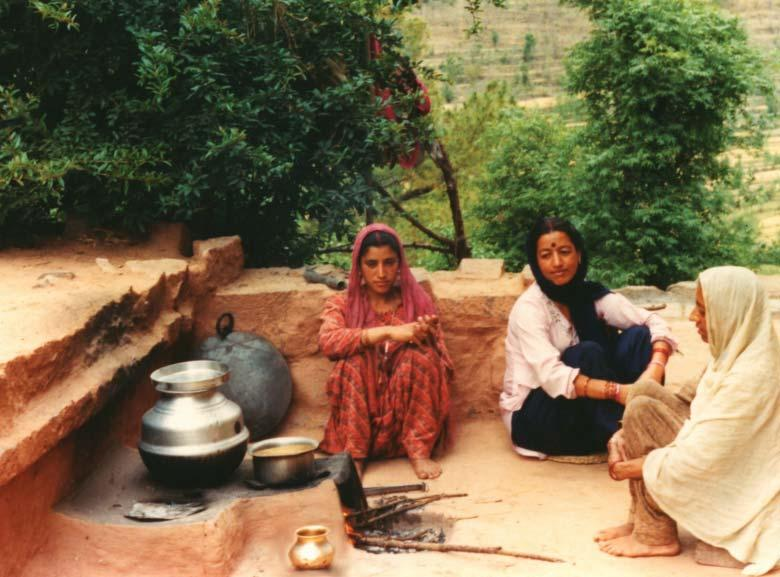
\includegraphics[scale=.34]{images/chap02-12.jpg}
\caption{An open-air kitchen}\label{chap02-fig12}
\end{figure}

Material for constructing a house is amply available locally. Good-grey coloured structural sandstone is available everywhere in this rugged hilly region. This stone can be finely hammer-dressed and chiselled. Because of the availability of good structural stone, very good professional stoneworkers are available in this region. Similarly, red-ochre and stiff clay is easily available in the vicinity of the villages. This clay has excellent binding and water-resistant qualities. When properly pulverised, sieved, mixed with binding material – cow-dung and the amply available pine needles (chalaroo) – and allowed to mature, it makes an excellent all-purpose gara. Good structural wood is, of course, scarce in this region, and people are obliged to use any type of wood – the resinous cheer pine, sal, semal (Bombax ceiba L.), tooni, kharak (Celtis australis L.), tali (Dalbergia lanceolaria L.), am or ambi (Mangifera indica L.), and others, depending upon the availability. Although none of these species is as good a structural timber as deodar, yet people make do with these species for the structural woodwork, which, obviously, is very simply made. Therefore, the use of wood is restricted only to the plain doors, windows and the roughly hewn square-cut joists, posts, beams, and so on.

The formalities for constructing a new house here are slightly different. After a suitable site is selected, the village Brahman is consulted. The Brahman prepares a horoscope of the proposed house, known as the griha-kundali, and finds out the most auspicious date and time for starting construction.

Initially, a piece of land is levelled and the foundation is dug to a depth of about half a metre. It is then filled with coarse gravel and levelled. This operation is followed by a brief religious ceremony. The owner of the proposed house brings the griha-kundali, wrapped in a red piece of cloth (kand) and places it within the layout of the proposed building. After performing pooja of the site (bhoomi-pooja), the foundation stone (shila) of the building is laid. The size of the foundation stone is duly prescribed in the griha-kundali. It is not necessary that the foundation stone should form a part of the structure. It has to be laid at the place prescribed by the Brahman, and could be laid even at a distance from the proposed house. In one instance, the size of the foundation stone (shila) as prescribed in the griha-kundali came out to be 17 angul (finger widths) long x 8.50 angul wide x 4.25 angul thick. This was required to be placed one hath (span of an open hand between the tips of thumb and little finger) and 210 angul away from the proposed house towards the agney-kon, that is, the southeast. On that occasion, the traditional musicians, locally known as the Turis, are invited to play auspicious musical notes. Gur (unrefined brown sugarcane jaggery) is distributed among all present on the occasion.

However, at times, people construct their houses according to the site condition and how it suits their means and requirements, without bothering much about what has been prescribed in the griha-kundali, based on the traditional vastushastra. For instance, in the griha-kundali of the house under study, the Brahman had prescribed that the proposed house should have rooms (biyoond) towards east with a fronting oblong enclosed veranda (chakhandee) and the entrance towards the west. However, what the owner constructed was a spacious four-roomed house facing southeast, with an independent kitchen and bathroom and fronting open veranda, but no chakhandee. Obviously, under the prevailing site conditions, one has to compromise on the prescriptions of vastushastra.

After the religious rituals are over, the actual construction begins. Since the soil stratum is normally hard and rocky, the excavation for the foundation is not taken deeper; about half a metre depth is considered sufficient. The foundation-trench is then filled with coarse gravels mixed with the locally available gritty clay, and thoroughly rammed. Over that foundation ‘concrete’, stone masonry work is completed without any offset up to the plinth level. The height of plinth is normally not more than 30 cm. Stones are laid in mud mortar. Above the plinth, the thickness of walls (bhitt or kandh) is normally reduced to about 30 cm to 45 cm after leaving an offset to the outer side for the outer walls. The internal walls are raised with offsets on both sides. All walls are made of properly hammer-dressed stones laid in mud mortar. Of late, some people are even using chisel-dressed and random rubble stones to enhance the architectural appearance of the houses. While no pointing or plastering is done on the external surfaces of walls as a general rule, since mud mortar used for laying stones is strong enough to bind stones together and keep the wall secure, yet people are increasingly opting for the use of cement, and one may find walls treated superficially with cement pointing. Affluent people are even using cement mortar for laying stone masonry, notwithstanding the fact that the local gritty calcareous clay is as good a bonding material as the cement mortar.

While the work of raising the wall continues, the doorframes and window frames are placed in position as per requirement. However, no opening is provided on the back wall, because in most of the houses, as in the present case, the back wall abuts on the hill profile, giving an illusion of the house emerging out of the hill slope as its organic part. Such houses are locally known as the daraba. The back rooms of such houses are pleasantly cool even during the severest summer months and comfortably cosy during winters. Normally the size of the door (dwar) is kept at 90 × 150 cm and that of the window (mori), at 60 × 90 cm. In the traditional house, one may find only a few windows, but a good number of niches (teeri) and recesses in the internal walls. The height of rooms in this area is abnormally high when compared to the ones in other places. Here the height is customarily kept between 3.00 m and 3.70 m so that the interiors may remain cool, even in summer. In these houses, generally fronting verandas are completely enclosed to form a large oblong room, called chakhandee, from where access to the rooms at the back is provided. The chakhandee is the most important portion of the house, where the inmates spend most of their waking hours. It is also used as a multipurpose living room. In some cases, in place of the chakhandee, an open veranda is also provided.

The flat roof (chat) of these houses is made of well-rammed impervious clay that keeps the interiors dry and insulated from the rains. For laying the mud roof, wooden joists (kari) are placed across the shorter span on the walls about 15 cm to 20 cm apart from each other. On these joists, 1.25 cm thick wooden planks are laid to form a ceiling (mairh). Dry grass or a lining of pine needles is provided over the mairh. Over that, a thick layer of gara is evenly spread. Finally, the entire roof is covered with a thick layer of rammed fine clay. A mild slope to one side is provided to drain out the rainwater. In some cases, instead of the flat mud roof, CGI sheet roofing (chadray-di-chhat) is also provided. If this is done, the outer walls are raised to form a parapet over the iron sheets so that these remain firmly pressed on all sides. The CGI sheets are laid with only a minimum slope to one side for the water to escape, so that the roof is virtually flat.

\newpage

The internal surfaces (and sometimes the outer as well) of the walls are plastered with mud mortar. The floor is also earthen, made of a thick layer of mud over the soling. The houses are whitewashed occasionally with makol. To prepare the whitewashing solution, the makol is dissolved in water and strained to separate insoluble residue. Some quantity of salt and gum or rice starch is then added to the solution. It is then ready for use. The exposed woodwork – the doors, windows, ceiling, and so on, are painted with red ochre with the traditional painting medium. To prepare the ‘paint’, ruddle (geru) is dissolved in water. That solution is then applied on the exposed woodwork and allowed to dry. When properly dried, a coat of mustard oil is applied to make the paint water resistant and lasting.


\subsection*{Housing Pattern in the Giri-par Area}

The rugged highland Giri-par (trans-Giri) area of Sirmaur district, is a mysterious country, where religious rituals are deeply steeped in sorcery and totemic orgies. Every aspect of life here is influenced by these and the predominating cult of Sirgul. Even in the construction of houses, the local belief-system has a decisive role to play. For instance, after the foundation has been ceremoniously laid, homemade liquor is distributed, and until the foundation for the entire building is dug and the masonry work completed up to the plinth level, day and night vigil is kept at the worksite, lest somebody plant a pernicious charm that may cause misery to the owner and his family. The owner even takes his meals at the construction site and keeps awake guarding the foundation through the nights with fire burning beside him. Apart from the owner or the baddhi, who is essentially a mason-cum-carpenter, no one is supposed to enter the area within the four walls of the proposed house until the walls reach the plinth level. During that period, even the labour engaged for the job is required to pass on the material – stones, mud mortar, and so on – from outside across the trench to the baddhi or the owner, standing on the other side. The baddhi is supposed to work from inside only. If any one violates this customary practice, the baddhi has the right to claim compensation, which may include anything the intruder carries on his person, be it a cap, a coat, a blanket, a shirt or a stick.

People also believe that a snake circles around the proposed house. Therefore, at the time of laying the foundation stone, the baddhi secretly lays the first two stones with a gap in between to ensure a safe passage to the ominous snake. Incidentally, the snake is popularly regarded as the lord of the subterranean sources of water. The possible reason for such belief may be this: since considerable hill-cutting is involved in the development of the site for a house in this area, there may be a possibility of exposing the underground flow of water that may cause problems for the proposed building. Therefore, leaving a gap between the stones in the foundation may be a naïve way to drain out such subsoil flow. The people have been following this age-old practise despite the fact that such a possibility may be very rare in this rugged and dry area. The author has found such a practice elsewhere, in such localities where the chance of encountering subsoil water is very remote.

In fact, most of the parameters of construction here are decided by the baddhi – a hereditary professional artisan. The baddhi is architect, engineer, mason and carpenter –allin-one in charge of construction and the final authority to decide matters related to the work. Normally, he is averse to any suggestion and does not entertain any change in his design. In fact, people also regard such interference ominous. The customary practice for the baddhi is to have his own team of two-three labourers to assist him. He normally undertakes construction work on a lump-sum contract basis, settled for a double or a three storeyed house, having a room on each floor as the unit. With an increase in the number of units, the unit rate is also proportionately increased. Such contractual conditions also imply that the proposed house shall be a double storeyed building, extending only linearly. House construction in this area is usually taken up in winter, when the baddhis and the villagers are free from their agrarian chores (Figure 2.13).

\begin{figure}[!htbp]
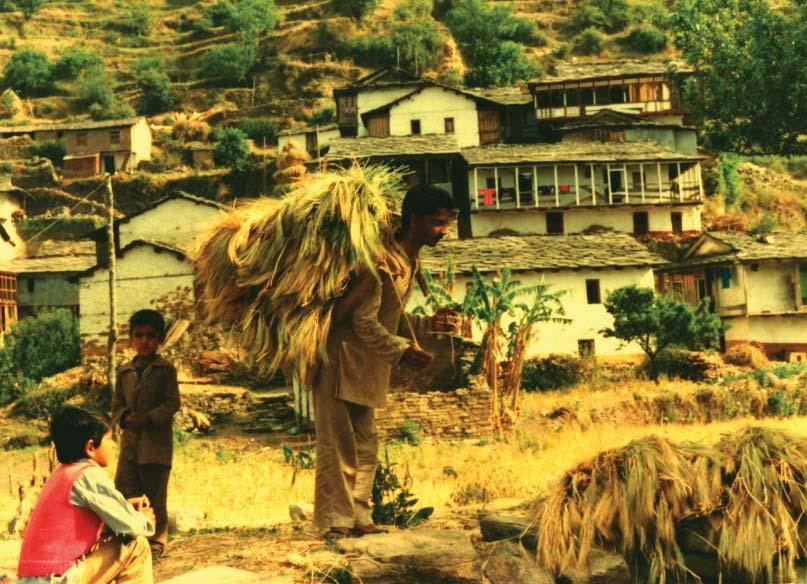
\includegraphics[scale=.34]{images/chap02-13.jpg}
\caption{A village setting in the Giri-par area}\label{chap02-fig13}
\end{figure}

For studying the housing pattern in the Giri-par area, a typical house of village Rajana was selected. This is a sizable and important multi-caste village of the Giri-par area of Sirmaur district, some 15 km of steep ascent away from Dadahu (Renuka). The village perched on a rugged mountain spur at an altitude of about 1530 m above sea level, is divided into two independent parts: the thickly populated upper part is called Uparala Rajana and the lower one is known as the Nichla Rajana. It appears that these two localities came into being to differentiate between the higher and lower caste communities. This caste-based segregative village pattern is a common feature of not only the Giri-par area, but one comes across that type of village setup everywhere in the interiors.

Besides arduous agriculture on unyielding terraced fields, people of this village are engaged in various other supplementary vocations, such as weaving, basket making, carpentry, black-smithy, and so on. Most of the villages in the Giri-par area of Sirmaur district, such as Rajana, are located on a higher altitude on the southwestern sunny aspect. Thus, summers are generally pleasant and bracing, but the winters are cold. It occasionally snows during winter, but the snow does not stay for long on the sunny slopes. In such a biophysical scenario, while normally the higher altitudinal temperate species are not found in this area, the trees of the lower altitude varieties are aplenty. Among these are the amaltash (Cassia fistula L.), ban (Quercus leucotrichophora A. Camus), brass, cheel, danri (Cedrela spp.), kharik (Celtis australis L.), sal, sani (Terminalia alata Heyne ex Roth.), shisham (Dalbergia sissoo Roxb.) semal, tooni, and so on. Most of these species are not structural wood, but people make do with these species for building their houses and making a variety of agricultural and household implements. The cheel, danri, kharik, sal, sani, shisham, semal and tooni are the common wood species used for building purpose (Figure 2.14).

\begin{figure}[!htbp]
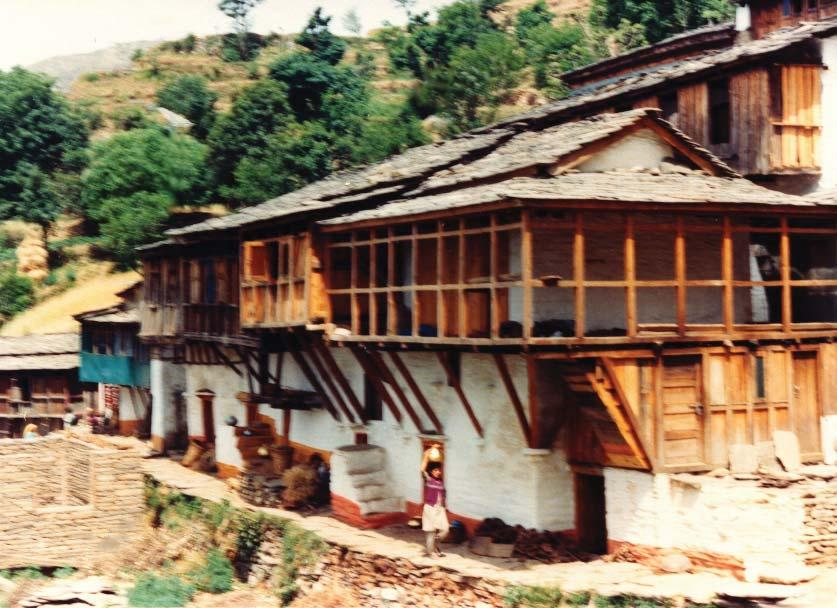
\includegraphics[scale=.34]{images/chap02-14.jpg}
\caption{A typical house in the Giri-par area}\label{chap02-fig14}
\end{figure}

The traditional houses at Rajana, as elsewhere in the Giri-par area, are made of stone, mud and timber to accommodate large extended or joint households. However, there is an increasing tendency among the affluent people to build ‘modern’ modular reinforced cement concrete (RCC) framed structures for their nuclear families under the expanding urban influence. Wood is being increasingly replaced by synthetic materials, like plywood, strawboards and modular plastic fixtures for almost all types of structural woodwork and indoor furniture.

As a rule, the houses in this area are built in a linear layout, along the contour facing the valley, at a location unsuitable for agriculture. Normally, the houses in this area have two or three floors. The dark and stuffy rooms are entered through the small doors, having an abnormally high sill. The height of this door does not exceed even 1 m, and one is obliged to bend on one’s knees to enter through it. Therefore, one has to climb up and step down to enter into the room. The rooms are without any window or ventilation, and if at all there is any, it is screened with pierced wooden blinders.

The houses are normally built as freestanding structures, clear and away from the mountain profile, which is generally buttressed by dry-stone breast. Normally, sufficient levelled ground is not available on the narrow and rugged terraces, but people develop plots by partial hill-cutting and filling. To retain the fill, dry-stone retaining walls that form the edge, are made on the valley side. Thus, a sufficiently wide-levelled ground is available for the proposed building, with ample frontage of about 3 m - 4 m. In that open space, a spacious sunken and paved rectangular courtyard is made, locally known as the gahana. The gahana literally means a threshing-yard but besides threshing, other agrarian chores are also performed here. On the outer edge of the gahana, about a metre wide and a half metre tall parapet is made which serves as the village thoroughfare, linking other houses at the same level.

The common materials used in the construction of houses are stone, local clay, slates and wood. The rough schist stone that is plentifully available in this area is neither good for masonry work nor can it be sliced into thin shingles. Nevertheless, people make use of it for construction purpose, but being very thick, using it for roofing purpose is commonly avoided. Therefore, for roofing purposes, slates are procured from such quarries in the area, where better quality of schist layers are available, as from village Bhalad, about 20 km away from Rajana. Generally, people make do with the locally available wood, but there are instances of importing deodar wood from the distant forests. The material required for construction is collected through community participation, locally known as haila lagana, that is, a call for voluntary labour. On the appointed day, the volunteers of all communities reach the owner’s place, where duties for collection and carriage of materials are assigned. For days, the volunteers are busy carrying stones, timber, slates, and so on. During those days, the owner feeds all the volunteers. When sufficient material has been collected, the owner arranges for a grand feast, in which rice, patinda, (leaven bread), gulti (mutton), ghee, shakar (jaggery) and homemade liquor are freely served. This institution of reciprocation through community participation is not only confined to house building, but most of the ceremonial events, social functions, and agrarian and farm activities are accomplished in this manner, throughout the interior of the Himalayan region. This institution has been known by different names at various places, for instance, it is known as dar, kewar or saret in Chamba, jwari in the Mandi-Kullu area, haila lagana and tthela in Sirmaur district, daruch or buara in the interiors of Shimla district, and so on.

After the site has been selected, the foundation is dug to a depth of about half a metre. Thick and flat schist stones are laid in the bed, over which dry stone masonry is started. Usually, the foundation is completely filled with stone masonry, but at times, the masons leave offsets also so that the width of the wall at the plinth level is about 50 cm to 55 cm. The plinth height itself does not exceed 15 cm to 25 cm from the surrounding ground level. Since the stone used for construction is poor quality schist, it cannot be dressed to proper shape, nor does it take any mortar. It is laid flat in irregular courses in such a manner that the faces of the wall are smooth and flat. The gaps and voids in the wall are packed with flints. Since this kind of masonry wall is vulnerable to all sorts of stresses and strains, it cannot be raised much higher without proper provision for a uniform distribution of the superimposed dead load. For that purpose, sturdy wooden wall plates (bad), tied with the cross-joists, are placed on both the edges of the wall. The vacant space within the framework is hand-packed with pieces of schist stone so that the surface is smooth. Such wooden frames are provided throughout the length of the wall after every 30 cm to 45 cm of schist stone courses. To ensure that the wooden frames remain gripped in position, these are joined with sturdy vertical wooden posts (thaili or shor), secured tightly to the wall on both sides. This type of wall construction technique is typical to the Giri-par area and the adjoining Jaunsar-Bawar area of the Dehradun district of Uttarakhand. A simple but striking example of such a contraption may be the tower-type temple of Shani Devta at Kharshali, on the way to Yamunotri in Uttarakhand (Handa 2003: 83). While the wall is being constructed, the doorframes are placed at proper places and niches and recesses (bhaiday) are provided in the wall, where required. Normally, no window is provided on the ground floor.

When the walls have been raised to a height of about 1.50 m, that is, the height of the ground floor, a wooden wall plate is placed on the outer edge. The rest of the wall thickness is covered with stones so that the top is uniformly smooth and levelled. Over that smooth surface, the floor joists are placed across the room over the shorter span. After that, the work of raising walls is continued until about 1.20 m height, that is, the height of the first floor. During that process, doorframes (dewad) and window frames are placed in position and niches and recesses made in the walls. Again, a wooden wall plate is placed on the outer edge, over which wooden joists are spanned. Beyond that, the sidewalls are taken up to form a gable for the roof (chhappar).

At the apex of vertical triangular walls, a ridgepole of rounded section is placed, over which rafters are placed at regular spacing. Over the rafters, wooden planks are fixed with nails. Over those roofing planks, thin slates are nailed, starting from the gable end to the ridge. At the ridge, an overlap of about 20 cm is given. A small opening (chhindwasli) is left on the roof at a proper place to serve as an outlet for the smoke. This opening can be closed when needed by sliding a slate over it.

After the external work is complete, the internal work is taken up, which starts with the flooring (maid) work. The floor level of the ground floor (mando) is usually kept a little lower than the plinth. It is finished with the flat schist stones. The ground floor is usually used as a cattle shed (obara or kando), but in certain cases, it may also be used for living, and mostly for sleeping and storage. In that case, the paved floor may be coated with mud and cow dung solution, which process is periodically repeated. For storage purposes, large wooden boxes, which usually occupy most of the room space, are made on the side along the walls. These storage boxes are known as kothar or badai.

For the flooring of the first floor (uprad), wooden planks are placed over the joists. No mud flooring is provided and the planks are left exposed. However, these are regularly scrubbed in the morning to make them look fresh and clean. The upper floor is the regular living area, where the family spends most of its time. Here, one room is earmarked as kitchen (rosyane). In one corner of the kitchen, a thick and large slate stone is firmly fixed on the floor over the mud cushion. On that raised platform, the hearth (chullhada) is made. The other rooms are used for living purpose. Sometimes, the loft (kandal) above the ceiling is also used for miscellaneous storage. To reach the first floor, an external masonry staircase is provided, which opens into a central room, open on one side. It is known as the jhee. Sometimes a cantilevered extension is also provided to the jhee. Access to the other rooms is always from the jhee.

The frames for doors (dwar) and windows are fixed in position during the construction of walls; then it is the time to fix shutters. People have devised a very simple but ingenious way to fix the shutters. For a door, the shutter is a thick one-piece plank of about 60 cm width. On one side of this plank, pivots are made at the top and the bottom. These pivots are inserted in the holes made in the horizontal members of the frame, or in the wooden sill and lintel, so that the shutter may turn on these freely. From inside, the door is closed by inserting a sturdy log of wood in holes made in the sidewalls, close to the shutter. A handle and a chain are fixed from outside. No window is provided on the ground floor. On the first floor, though the windows are horizontally of large size, but the openings in them are very small and narrow, with most of the openings completely blinded with crudely perforated wooden planks. The perforations in the blinders may admit only dim and defused light and minimal fresh air. The flat surface of these wooden blinders is carved with folk, geometrical, floral, faunal and figurative designs.

By way of finishing, the walls are plastered from both sides. The plastering medium is prepared by mixing pulverised earth and cow dung together. The mixture is then allowed to remain in water for some days to turn into gara (mud mortar). When the plaster is dry, whitewashing is done with the locally available makol. White washing may be repeated occasionally.


\subsection*{The Jaunsari Housing Pattern}

Before discussing the housing pattern of the Jaunsari area, it may be necessary to define the term ‘Jaunsari’. The rugged mountainous tract spread over the Sirmaur district in Himachal Pradesh and the Jaunsar-Bawar paragana of Dehradun district in the catchment of the Tons river, may generally be defined as Jaunsari not only for the geophysical consideration, but also because this entire area forms an integrated ethnic, socio-cultural and religious entity centred on the cult of Mahasu. Further, there is a distinct similarity in the domestic and religious architecture of this area. Nevertheless, the people of Jaunsari region belong to the same Khash ethnic stock, to which belong their counterparts in the Giri-par part of Sirmaur district, and are equally steeped in sorcery and totemic practices. Thus, many customs and practices of this region may be common with the Giri-par region. The people of this region have been notorious for pilfering deodar wood sleepers, which the forest contractors have been floating down the Tons, to build their houses. That method of transporting sleepers by floating them in the river is locally known as ghal. For this reason, while the same species of wood is found in this area as in the Giri-par area, but the houses here are largely wooden, with extensive use of mostly pilfered deodar wood.

For studying the traditional domestic architecture of this area; two typical houses, one of village Kamrao, and the other of village Jadi, both in the Tons basin were selected. Village Kamrao is situated about 40 km from Paonta on the Paonta-Shilai road in the Kamrao sub-tehsil in Sirmaur district on the right side of Tons. Village Jadi falls in the Jaunsar-Bawar paragana of Dehradun district towards the left of Tons in Uttarakhand. This village is located about 13 km from Chakarata on the motorable road to Tyuni and Hanol.

Village Kamrao is spread in three patti (hamlets): Chowki, Shlana and Manana. These patties are located distinctively apart at three levels. Of these, Chowki or Kamrao proper is possibly the oldest locality. The village, perched on the steep slope of a rugged mountain range facing south, has a strange nostalgic charm about it. The neatly built multi-storey houses laid linearly along the contours, with meandering stone-paved lanes and bye-lanes, exude something mysterious and ominous, which is heightened manifold by the totemic reputation of this area. The people of Kamrao are known for their fondness for substantial houses. For instance, the house of Mohar Singh at Manana had 42 households (Singh 1966 b: 1) substantial house is locally known as ghar, and a modest one, as the tali. In Chowki, most of the houses are three storeyed, while in Shlana, these are two or three storeyed and in Manana, almost all houses are double storeyed. Single storey houses in Jaunsari area are rare.

To construct a house, the owner first plants four wooden pegs on the four corners of the site selected for the purpose. Then, an auspicious red raw cotton thread (paranda or mauli) is tied around these pegs to demarcate the extent of the covered area. Within that demarcated site, a chela or a Brahman (mostly a Khash-Brahman) conducts purificatory pooja. Thereafter, for eight days, one male member of the family stays guard against any rambling evil spirit. A makeshift shelter may also be made at the site for the guard to sleep. In the meantime, arrangements are made for the collection of materials – wood, stone, slates, and so on. The stones and slates are mostly available around the villages in this area and the people do not have to go very far for these items. They collect these materials through community participation. The owner is obliged to serve the volunteers evening meals together with sur (the homemade liquor). Mutton is generally cooked and served on such occasions. However, people have been finding it difficult to arrange for wood, for they do not have the customary bartandari right to get wood from the specified forests at concessional rates. Perhaps, that may be one of the reasons that drove people to pilfer wood, especially deodar wood, from the ghal in the Tons (rarely also from the Giri River), but they never confess to it. However, with stringent control on pilferage, people are gradually opting for ‘modern’ construction materials and techniques.

Customarily, no community participation is solicited for labour required during the construction. The family members usually provide manual labour for that purpose. Because, the local people are usually not available for that purpose, those who can afford hire labour from outside. The ‘immigrant’ Nepali and Bihari labourers are now available in plenty for the job. In fact, it is now difficult to get local people for any type of unskilled manual work of construction, horticulture and agriculture in Himachal Pradesh, and that void has been filled by the immigrant labour, mostly Nepalis and Biharis.

To start construction, the foundation is dug to a depth of about 80 cm. The masonry work in the foundation is done with the stones laid in mud or lime mortar, and continued to a height of about 20 cm to 30 cm above the surrounding ground level. The height of the walls for the ground floor or obara is raised to about 1.80 m. People use dressed and undressed stone for building purposes, depending upon the owner’s financial status. The obara may have one or more rooms, depending upon the economic condition of the household. If there is more than one room, one of those may be used for tethering cattle and the remaining, for storage, but usually obara is used for tethering the milch cattle only. The flooring of obara, locally known as the dhain, is also paved with large flat stones. Depending upon the requirement, the dhain may be covered with a coat of mud and cow-dung solution. The surfaces of walls are also plastered with the mud and cow-dung gara. The obara has only one entrance door, with no window (atali) or ventilator (chhandwalie). The entrance door is not only small and narrow (about 120 cm x 90 cm in size), but it also has an elevated sill so that the filth and water do not enter into the obara. Therefore, one has to strain and bow low on one’s knees to get into the room. This door also provides access to the stepladder to the upper floor, and one is supposed to take off one’s shoes before climbing the stairs. The door is usually a single piece thick wooden plank with one side pivoted, fitted into the doorframe. To close it from inside, a large wooden log (aghal) is inserted across it in the holes on the sidewalls. When this door is shut from inside, the entire house is completely closed to the outsider. Such foolproof security measures were mandatory among the strife-ridden Khash social setup since Mediaeval times.

In this context, a popular tradition of the area informs us that once, long ago, the people of Kamrao earned the animosity of the Thunds, a village community in Jubbal state, over some issue. This turned into protracted skirmishes between them. In order to protect themselves and their houses from the ravaging attacks of the Thunds, the people of Chowki resolved that each night, one able-bodied person from each household should keep vigil for a possible surprise attack by the enemy. They also decided to bring about modifications in the design of their houses, and to that end, only one narrow and small entrance was provided for a house. Thus, an intruder, while entering the house, had to strain his body and bend on his knees; this made him vulnerable to attack from the inmates (Singh 1966 b: 7-8). This is only one tradition of inter-clan animosity, but such inter-clan rivalries had been numerous during Mediaeval times among the different Khash warrior clans, known as the khoond. Those feuding khoond became known as the Shattha (or Shatthi) Khoond and the Pattha (or Bashi) Khoond (Handa 2004b: 69). Most of those rivalries ended in sanguinary episodes.

No stone is used for the walls on the upper two floors – second storey, called manjh, and the third storey, called baud. The manjh and baud are used exclusively as living floors. These are made entirely of wood. The use of iron nails is kept to a bare minimum in woodwork, in the traditional style of construction for fixing the beams (baih), planks, and so on. These are generally lap-jointed or dovetailed in a very professional manner. The woodwork in some of the houses in this area is so perfect and well-jointed, especially the internal woodwork, that one is amazed at the degree of skilled workmanship of the traditional local baddhis. Although people would prefer deodar wood for the woodwork, they could use other species under compelling conditions. Obviously, the baddhi employed on the job has to be a carpenter and a mason rolled into one, which normally is the case. Each of the upper floors has a spacious central room (chanbara) and a covered projected veranda (choh) or balcony (tung). The choh or tung forms an integral part of the chanbara, making it very spacious and an all-purpose living area for the household. Along the sidewalls of this room, large wooden boxes, locally known as the kuthar, are permanently inbuilt for storing grains. Few cupboards may also be provided in the inner wooden walls of the living rooms, where articles of daily use are kept.

In one part, partitioned off from the chanbara, the kitchen (rasoi) is situated on the manjh or the first floor. In some cases, the kitchen may be an entirely independent room adjoining the chanbara (the central room). The chullha (hearth or cooking range) is built in a corner over a thick and large slate stone platform laid over the earthen cushion. The large and thick slate stones are also placed against the wooden walls (bhitt) for protection against fire. No chimney is provided above the chullha for smoke to escape. In some cases, the kitchen is made on the second floor. In that case, a small ventilator (chhandwalie), with a movable slate shutter, is provided on the roof. The kitchen fire is always kept smouldering and is ready whenever required. In fact, extinguishing fire in the hearth is regarded a bad omen throughout the Himalayan region. Kitchen utensils are also kept very clean. A separate space may be provided for keeping water vessels. None of the houses has a bathroom or a toilet.

With the cantilevered veranda and balconies on the upper floors, the manjh and baud of the Jaunsari house are far more spacious and larger than the ground floor (obara). In the upper storeys, atali with sliding panels are normally provided; an atali is only an apology for a window, except for a small and stylised aperture, there is no opening in it. Customarily, access to the upper floor is only provided internally from the obara through a stepladder (shir), which opens into the spacious central room (chanbara) on the first floor, and thence to the second floor through the trapdoor, with no access from outside for security reasons. However, lately people are also opting for external portable ladders.

Ordinarily, no ceiling is provided on the top floor, and the wooden under-structure of the roof is clearly visible. The laying of the roof formally marks the completion of the house. On that occasion, the baddhi climbs on the ridge of the roof and sits there to claim the customary obligation for the service rendered by him. He stays put until a satisfactory offer is made to him in cash and kind, besides the settled contractual payment on unit basis, discussed earlier in the context of Giri-par housing pattern.

For finishing and painting, the exposed woodwork is treated with a coat of ochre solution made by dissolving geru (ruddle/ochre) in water. When it is completely dry, mustard oil is rubbed over the coated surface with a piece of cloth. That gives a rich ochre coloured finish to the house. It is believed that the ochre-and-mustard oil coating protects the woodwork from termites and other harmful insects. The wooden floors (pharkion) are cleaned and scrubbed daily and kept meticulously clean. Once a week, these are scrubbed with cow urine (gontar) which is believed to be a disinfectant. The people of this area are very proud of their houses and maintain them with loving care. The houses built decades ago look new, as if made recently. Credit for such meticulous maintenance of their houses goes to the womenfolk of the area.

It is customary in this area to construct an independent small wooden kiosk, standing high above the surrounding ground on four sturdy legs in an open corner of the fronting angan. That kiosk is locally known as the tand. The wooden walls of this cabin are made of sturdy wooden battens, placed closely apart to keep the interior adequately ventilated, but protected from vermin. This cabin is made secure with proper roofing and door. The tand serves as storage for the maize cobs, which get naturally dried in storage and well protected from rats and other rodents. The author has seen such storage kiosks in the Uttarkashi district of Uttarakhand also, of which, the one at village Kharshali, 35 km from Parola, in the Uttarkashi district is interesting. Located on one side of the open ground, this sizable kiosk is made of sturdy deodar wood planks and logs and covered with a fine slate roof. This kiosk, popularly known as the bhandar, belongs to Mahasu Devta at Hanol. In this bhandar, the annual tribute of the Mahasu Devta, known as the koot, is stored. People pay koot in kind, in the form of coarse millet, mostly koda or mandua.

Now, the other Jaunsari house at Village Jadi towards the left of Tons is taken up for discussion. Located about 13 km from Chakarata\break (Figure 2.15) on the motor road to Tyuni and Hanol, this village is a small yet beautiful Khash (Khashia) village in the Jaunsar-Bawar area of Dehradun district of Uttarakhand, opposite the contiguous part of Sirmaur district in Himachal Pradesh, on the right of Tons River. Not only is the housing pattern of the major eastern part of the Giri-par area in the Tons basin of Sirmaur district carried over to this part, but the entire socio-cultural and religious fabric of the entire area is also the same. In fact, once this area formed a part of the defunct Sirmaur kingdom, now incorporated into the Sirmaur district. Therefore, the Jaunsari housing pattern, also holds good for the entire housing pattern in the adjoining Shilai area (or the major eastern part of the Giri-par area) of Sirmaur district.

\begin{figure}[!htbp]
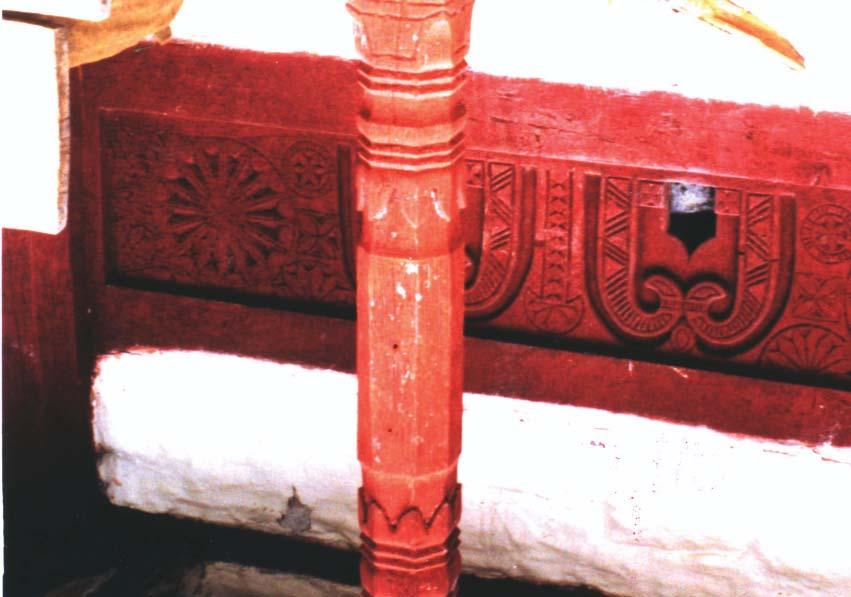
\includegraphics[scale=.28]{images/chap02-15.jpg}
\caption{An artist’s impression of the rural setting, Chakrata, Dehradun (Photograph by Author of painting by Dr. M. Jain.)}\label{chap02-fig15}
\end{figure}

Jadi village is a typical example of the Jaunsari archetype, distinguished by two or more storied houses, built in linear form along the contours of the rugged mountain slopes, similar to the ones that are found in the adjoining part of Sirmaur district. The people have planned their houses in a manner that suits their agro-pastoral requirements. The ground floor, which at times abuts the mountain profile on the back, is meant to keep cattle, goats and sheep.

The upper floors have wide verandas facing the valley, with the rooms set on the rear in a linear formation. The rooms are generally inadequately ventilated and dimly lighted. The doors are very small and narrow and so are the narrow horizontal windows (atali) covered with wooden blinders to allow only restricted light and air through the stylised slits. However, these serve well to insulate the rooms from the external chill during the winters. A wide and open space, directly connected to the veranda, is left in the middle between the living rooms. This open space (chanbara) and the fronting veranda is the busiest part of the house. At times, the veranda is enclosed totally or partly according to the individual need of the household. The open verandas are used for drying and storage of grains, performing domestic chores and the occasional family gatherings. As a matter of tradition, all the exposed wooden structural members, doorframes, shutters, posts, pillars, railing panels, window frames and panels, and so on are tastefully carved and coloured with red ochre (Figure 2.16).

\begin{figure}[!htbp]
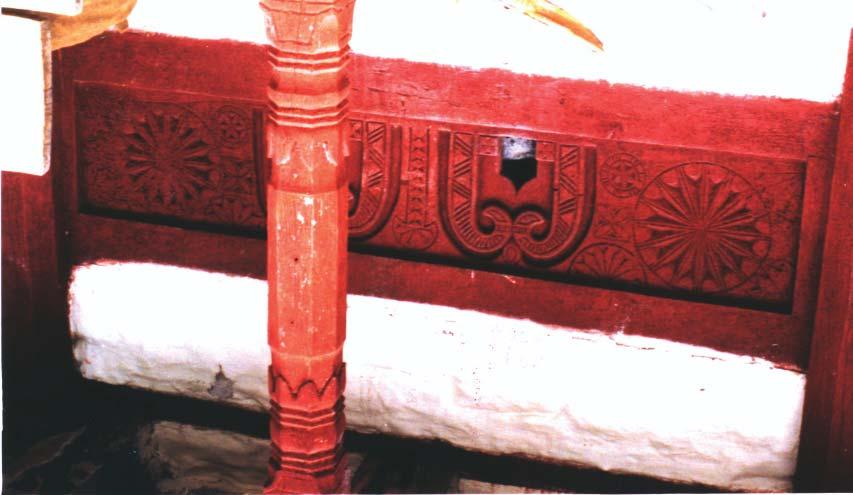
\includegraphics[scale=.3]{images/chap02-16.jpg}
\caption{A carved window of a Jaunsari house at Jadi}\label{chap02-fig16}
\end{figure}

The houses are invariably provided with gable roofs and covered with locally available coarse shingles. As is the general practice, an adjustable escape gap is left on the roof over the kitchen, exactly where the hearth is located, to drive away the smoke. The ridgepole on the residential houses is plain and simple. It is held sacred and laid on the roof with due ceremony and sacrifice. However, those rites are not as elaborate as for the temple. Although gabled roofs may be common, both to a residential house and a temple, there is a subtle difference in the overall structural arrangement of the two.

While the door must be placed in the centre under the gable for the temple, in a residential house, the door is invariably on the lateral side.

What makes the Jaunsari house in Uttarakhand look different from its counterpart in Himachal is the variation in the construction of the wall. While the houses at Kamrao in Himachal Pradesh, generally have stone masonry walls for the ground floor only and the wooden panelled walls for the upper floors, the houses at village Jadi in Uttarakhand have stone masonry load-bearing walls for the entire structure, similar to the ones that are found in the Giri-par houses at village Rajana, noted earlier. What is common in the Jaunsari houses (Figure 2.17) on both sides of the river Tons is the fact that the indispensable front threshing yard is generally, conspicuously missing in these houses. That may indicate that the cultivation of cereal crops, which need threshing to remove chaff from the grains, has remained marginalised in this rugged area, and the people have been cultivating such crops for which a regular threshing yard is unnecessary.

\begin{figure}[!htbp]
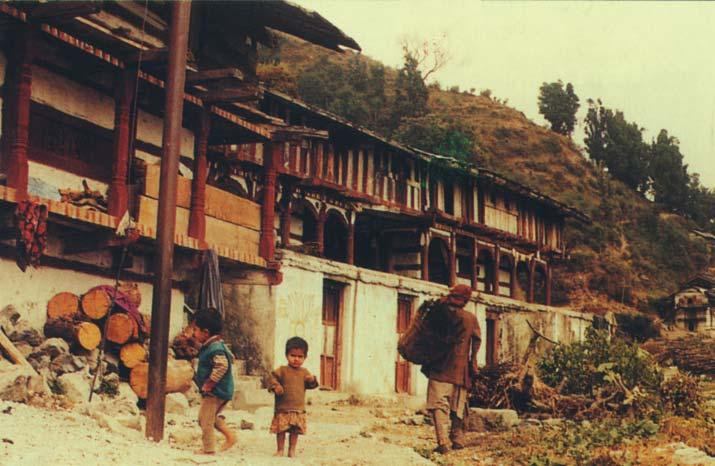
\includegraphics[scale=.37]{images/chap02-17.jpg}
\caption{A typical village house at village Jadi}\label{chap02-fig17}
\end{figure}


\subsection*{The Housing Pattern in Kyarda Doon}

Kyarda Doon is the traditional name of the area which is now popularly known as Paonta Doon, for the village Kyarda. It is now a small roadside village on the Paonta-Nahan road. For instance, the house type in the Jaswan Doon is similar to the one in the section entitled Lowland House in the Temperate Setting that has been discussed, and what is found in the Doon of Solan district does not differ much from what has been discussed in the section entitled Housing Pattern in the Doon Highlands. However, here the residential housing pattern in the Kyarda (or Paonta) Doon, has an entirely different ethno-cultural and geo-climatic context and different biophysical conditions prevail.

\vskip 2pt

The Kyarda Doon is generally characterised by subtropical climatic conditions, with very hot summers and mild winters. The floor of Kyarda Doon is a vast undulating tableland, with stretches of flat land spread on the banks of both the rivers Markanda and Bata. Both these rivers, though seasonal, keep flowing even in an emaciated state during extreme summer conditions, but virtually inundate the entire doon during the monsoons. Both these rivers originate from somewhere in the middle of the Dharti Range, but diverge in diametrically opposite directions: while Markanda River flows south-westwards, the Bata River continues to flow towards the southeast and pours into the Yamuna at Bata Mandi near Paonta. The villages, interspersed by the thick and grassy jungles of various species, are situated here on the higher and undulating or mildly inclining terraces of the conglomerate alluvium, not suitable for agriculture. Most of the major villages of the area are well-connected with urban centres on all sides by several all weather roads, crisscrossing through various villages, but the two highways – Nahan-Paonta-Dehradun road and Nahan-Kala Amb-Ambala road are the most important ones. Besides, all the villages in the area are interlinked with cart roads, and most of the villagers have their own bullock carts.

\vskip 2pt

The present inhabitants of Kyarda Doon are not native to the area. Possibly, this area and the vast Siwalik foothill tract remained dominated by the ancient Kulinds or their later descendants, the Kunets. Structural evidence of the old settlements is plentifully available, embedded among the thick bushes and massive trees in the jungles almost everywhere in this area to indicate habitation and activity in the remote past. The author had a chance to explore this area extensively and found habitational evidence deep in the forests not only at Sirmauri, Tal and Nagnaun, but also at Mirpur Kotala, Amboya, Parduni, Bias, and other places. What were the circumstances that compelled the earlier inhabitants to migrate are difficult to know.

\vskip 2pt

Devoid of human involvement and activity, the Kyarda Doon turned into a vast stretch of thick and wild jungle, abounding in all sorts of wild animals, including panthers, tigers, elephants and game animals. There are thick forests even today, but panthers and tigers are rare now and elephants are extinct. The other communities are evenly distributed in the entire doon.

\vskip 2pt

For this study of the traditional housing pattern in the Kyarda Doon, the author selected two typical houses, one belonging to the Labana community and the other, to the Koli community. The houses of other communities are not different from the ones of these two communities. Since the Labana settled in the Kyarda Doon from the adjoining tropical plains of Punjab, they also brought with them their traditions, manners, belief-systems and housing style. All those traits are clearly reflected in their lifestyle and dwellings, in which grass and jungle wood have a pre-eminent role.

Under these abovementioned broad parameters, economic and functional considerations have also greatly influenced the form and style of the traditional housing pattern. The choice of material for constructing walls and roofs depends upon the economic status of the owner. Besides, the purpose for which the house is to be built is also a major deciding factor. Since the land has been no problem for constructing a house, the traditional houses in the Kyarda Doon are essentially single storeyed structures located widely apart from each other, mostly in irregular linear formations on such higher terraces not suitable for agriculture. These houses spread horizontally rather than vertically, and almost every house has a well-maintained spacious fronting courtyard and sufficient open space around, not only to grow flowers and vegetables, but also to have a variety of fruit bearing trees like banana, papaya, guava, mango and varieties of citrus. Those houses may be broadly be classified into three types:

\begin{enumerate}
\item Mud-built thatched dwelling,

 \item Masonry structure with thatched roofing, and

 \item Masonry structure with CGI sheet roofing.

\end{enumerate}

\newpage

\subsection*{\textit{Mud-built Thatched Dwelling}}

The mud-built thatched dwellings are traditionally associated with the Labana. As a majority of them inhabit the main doon to live in isolated single large room (kotha), the four walls are made of mud and covered with thatched roofs (chhappar). These huts are mostly made of locally available material, boulders, earth, jungle wood, bamboo, twigs, grass, and so on, almost entirely without using iron nails and other fixtures. No skilled artisan or external labour is required to build such dwellings, but the family members, men and women work together to make their home cosy and comfortable, born organically out of the soil.

To make such a hut, an elevated plain piece of land is selected. The work of excavating the foundation is normally started without any formal ritual. The foundation (neev) is not dug beyond a depth of 45 cm to 60 cm. It is then packed with boulders up to the ground level. Over it, a plinth course of random stone masonry is laid in mud mortar. There are two options for fabricating the superstructure of a kotha.

The simplest way to start the kotha superstructure is to erect four sturdy jungle wooden logs of equal height, with forked tops on the plinth, one at each of the four corners. Two similar but taller logs are planted in the middle of each lateral plinth. A ridgepole is spanned on the taller logs, and similar horizontal logs are secured to the forked ends of the verticals planted on the corners. On that contraption, wooden or bamboo rafters are spanned. Thus, the infrastructure for the thatched kotha is complete. What remains to be done is to place the prefabricated thatched roof (Figure 2.18) on the rafters and provide four walls, made of thatch properly stuffed into the bamboo frames. The other option is to embed the four corner logs in the four earthen walls.

\begin{figure}[!htbp]
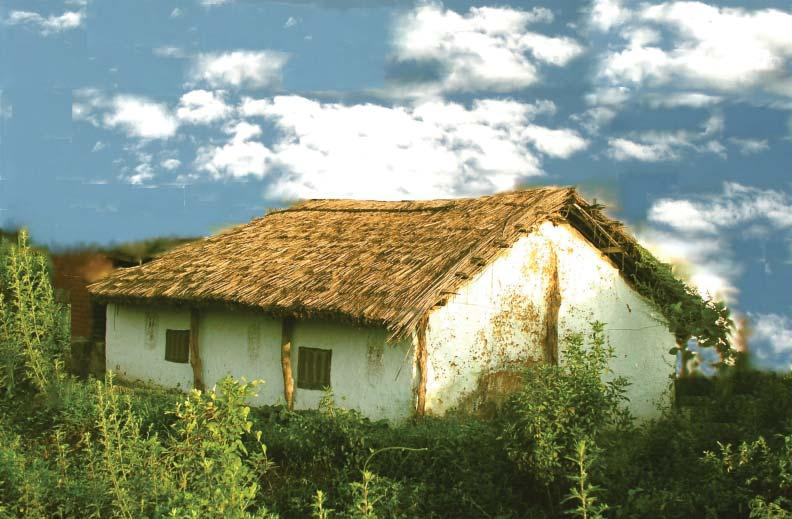
\includegraphics[scale=.32]{images/chap02-18.jpg}
\caption{A thatched roof dwelling in the Kyarda Doon}\label{chap02-fig18}
\end{figure}

However, further improvement over the completely thatched kotha is the one made of four earthen walls and covered with prefabricated or built in-situ thatched roof. For such kotha, over that plinth course, 45 cm to 60 cm thick earthen walls are raised to make an all-purpose large rectangular room of about 8.50 x 3.50 m floor area. To make the earthen walls, locally available clay is first sieved with the chhanni. An appropriate quantity of rice husk, chopped rice chaff or grass is added to it as a binding medium. The mixture is then well pulverised and thoroughly kneaded to form a pliable mass of mud of the desired consistency.

After the mud is ready, two sturdy wooden planks are positioned horizontally on the plinth course, spaced apart to define the width of the proposed wall. The space between them is filled with mud. To make the filling compact, it is thoroughly rammed with mungaree (large wooden mallet). At times, small pebbles are also embedded in the fill. The process is repeated by horizontally shifting the wooden planks from one place to the other until one course of the filling is complete. In that manner, course over course is piled up until the longer walls reach the desired height, which is normally about 2 m.

The shorter sidewalls are raised further to a height of about 1 m to 2 m to form the gable. Such earthen walls are known as matkanda. At times, to make the gable, only the earthen pillars are raised in the middle of the sidewalls to support the ridgepole, while the remaining part of the sidewalls is kept at the same level as the longer walls.

While the process of making matkanda walls is in progress, a gap for the main door (keewad), which opens into the fronting spacious courtyard, is left normally in the middle of the long wall. The door is never provided under the gable for residential houses. This door is the only opening in the hut, but there is hardly any problem of air and light in the hut, for the gaps under the gable, between the four-walls and the roof, and the thatched roof take care of that rather effectively, and diffused light and air is amply available inside. Therefore, the interior of such a hut remains very airy and reasonably lighted (Figures 2.19 and 2.20).

\begin{figure}[!htbp]
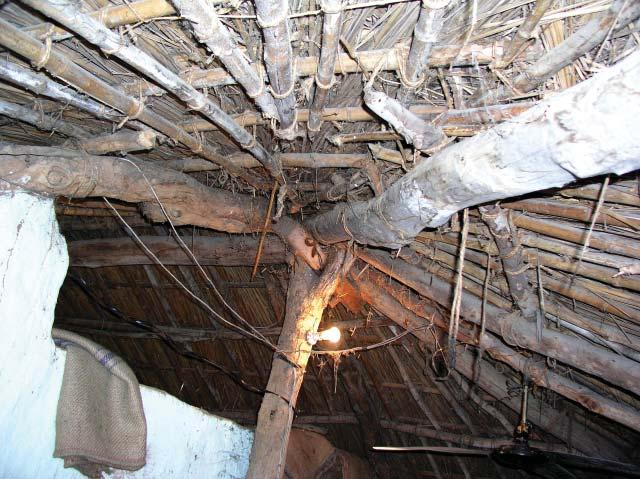
\includegraphics[scale=.35]{images/chap02-19.jpg}
\caption{The underside of a thatched roof}\label{chap02-fig19}
\end{figure}


\begin{figure}[!htbp]
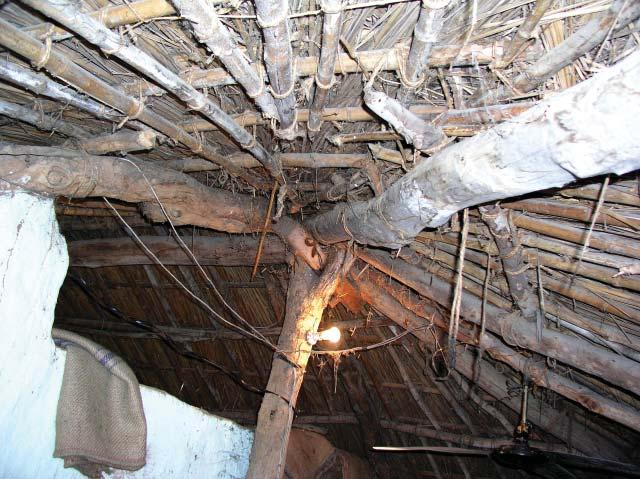
\includegraphics[scale=.35]{images/chap02-20.jpg}
\caption{Detailed view of the supporting logs of a thatched roof}\label{chap02-fig20}
\end{figure}

When the matkanda walls are ready, a round wooden log is placed on the apex (magri) of the sidewall or the earthen pillars to serve as a ridgepole (balla or ballee). To make the ridgepole secure atop the gable, it is fixed to the base with a wooden contraption, called korve and kanta. In case, there is fear of the balla sagging due to a longer span, it is propped up by wooden supports (thambi or tham) erected in the mid-span. Rafters (balla or ballee) are then spanned, with their top ends resting on the ridgepole and the lower ends resting over the longer walls. Care is taken to extend the rafters by about half a metre beyond the outer face of the wall to make a projected gable-end (lotiya).

Mostly logs of sandan or sal are used for this purpose, but use of bamboo is also seen in several houses. To fix the rafters firmly, these are tightly secured with the ridgepole by sturdy maljan (Bauhinia vahlii Wight and Arnott) vines. Over these rafters, thin wooden scantlings or split bamboo battens are firmly tied with the maljan vines to form a sort of framework (badondh). Once the framework is complete, the actual roofing process is started. Normally this work is done by family members themselves, but the people skilled in laying thatched roofs are also available.

These varieties of grass are amply available in the area. The base layer (neeran) which is about 3 cm thick is systematically spread, starting from the gable end to the ridge (modian). Over that base layer, about 15 cm thick layer of grass is spread in a similar manner. Sometimes, a framework of thin bamboo strips is also provided over the grass to make the roofing a compact single mass. Once the laying of grass (and optional bamboo framework) is complete, the layers are carefully tied with ropes to the wooden or bamboo under-structure so that the roof becomes a tightly secured compact mass, lest it is blown away with the wind. The ropes used for tying the roof are also locally made of bhabhar or baga grass. Such rope is known as ban. Thin and stronger ropes are also made from the fibre of mulberry (Morus alba L.) for tying thatched roofs and for various other purposes. The thin flexible twigs of mulberry are also used for preparing tokari (baskets) and chhaba (flat baskets) for carrying building material.

The single door (keewad) of the hut is made of locally available wood. The doorframe (chokhat) may be with or without sill (sardal), but the entrance is always kept higher from the floor level of the room. A single-leaf pivoted shutter is provided, with a horizontal log (ballee) attached to it from inside to close it. The external locking arrangement is the only metallic fixture in the entire structure.

After the hut is complete from outside, internal work is taken up. The floor of the hut, which is about 15 cm to 30 cm above the surrounding ground level, is made of locally available small stones, pebbles and grit, made compact with the mungaree. Over that soling, a thick layer of moist earth is laid, made compact by vigorous ramming. The surface is then finished with a cow dung solution, and the walls are finished after mud plastering. Whitewashing or colour washing may be done with locally available coloured clays, and repeated occasionally.

The kotha is the multipurpose living room, where, in one corner, an earthen chullha is made for cooking meals. At this time, the kitchen (rasoi) area is set apart from the living area within the kotha. For that purpose, a jalee (screen) is appropriately fixed as a curtain or partition wall. This jalee is made of stalks (Figure 2.21) of sarkanda, kahi, kan or kans (Saccharum spontaneum L.) or bamboo strips tied into a framework.

\begin{figure}[!htbp]
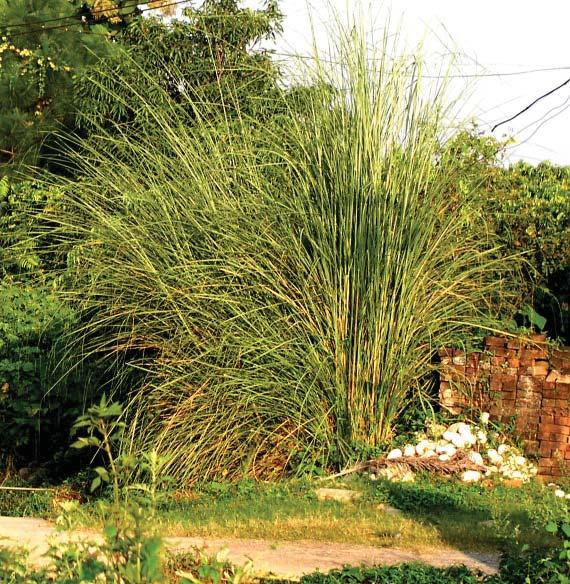
\includegraphics[scale=.33]{images/chap02-21.jpg}
\caption{The Sarkanda (common spear grass) that grows wild in the Kyarda Doon}\label{chap02-fig21}
\end{figure}

In the kitchen area, a stand for keeping water pitchers (gharonchee) is also provided and niches (ado) are made at appropriate places in the wall. Sometimes, a large earthen container (kothi) for storing grain is made as a divider between the kitchen and the living area. To make the thin walls of such a container also, bamboo strips or the split stalks of kahi, kan or kans are tied together to form a framework. That armature is erected in position to serve as reinforcement. Lumps of stiff gara are then filled in the gaps of that armature. When the filling is semidry, the framework is tightly plastered on both sides with thick coatings of gara, and finished with the clay-cow dung solution. Thus, the ‘reinforced’ mud wall is complete. Such a wall can be made of any thickness to serve various purposes: it can be used as a thin partition wall, or in a staggered form to make cupboards, containers and silos (Figure 2.22).

\begin{figure}[!htbp]
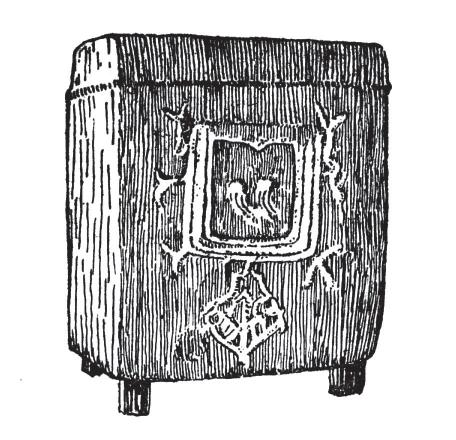
\includegraphics[scale=.35]{images/chap02-22.jpg}
\caption{An earthen container (Kothi) for storing grains}\label{chap02-fig22}
\end{figure}


\subsection*{\textit{Masonry Structure with Thatched Roofing}}

The houses made of stone or brick masonry walls are not a one-room affair, as in case of the aforementioned kotha, built of matkanda and chhappar. These are multi-room single storey houses, which have assimilated the broad layout features of the houses in the Doon highlands and the roofing style of the kotha of Labana. Traditionally, most of such houses are owned by the Koli, who inhabit the wild and undulating area along the Markanda River. Despite the rough topography of the area, the houses of Koli are widely spaced apart in a linear formation. However, the well-kept courtyards and cultivated surroundings, so common around the thatched huts of the Labana, are conspicuous by their absence here despite ample open space around the houses. However, a few papaya and banana plants may be found here and there.

A typical Koli house (Figure 2.23) essentially comprises a large rectangular room with an enclosed veranda in front, but such a dwelling unit has ample scope for lateral expansion on both sides. Thus, a small room with a fronting veranda may be added to the existing structure on one side, and if needed, a veranda may be extended to the other side to make an independent kitchen. In any case, the veranda is always enclosed, looking like an elongated room with entrance door and windows or honeycombed pigeonholes. Each room has an independent door from the veranda. Normally no window is provided on the sides, for the house may need lateral expansion subsequently, but there are windows on the back wall and in front wall of the room. The front windows open into the enclosed veranda, and, thus, these hardly serve the intended purpose. Although the people do not care much about orienting the main entrance of the house, yet they consider a south facing entrance inauspicious.

\begin{figure}[!htbp]
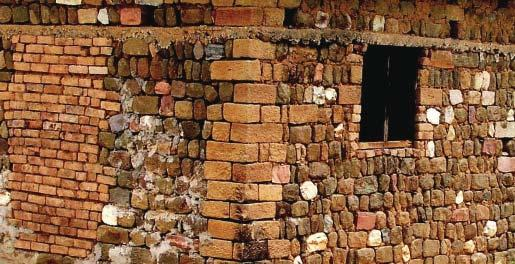
\includegraphics[scale=.53]{images/chap02-23.jpg}
\caption{A brick and stone conglomerate wall of a Koli house}\label{chap02-fig23}
\end{figure}

Unlike the institution of voluntary community participation for constructing a house, as has been noted in the Himalayan interiors, or a house built by the family members themselves, as in the case of the Labana, the people desirous of building a house here normally hire skilled and unskilled labour. The masons undertake masonry work and the carpenters do the woodwork, and they are paid in cash on pre-settled terms. They sometimes assist the owner in designing his house. The two-in-one traditional complementary institution of the hereditary baddhi is unknown in this area.

Unlike the Labana, the Koli observe necessary religious rituals before starting construction of a house. The village Brahman is consulted to find out an auspicious day. Usually people regard Navaratra as the most opportune time to start house construction. On the mahurat day, gur or shakar is distributed before digging the foundation. The foundation is dug to a depth of about 60 cm to 90 cm, depending upon the underlying strata. It is then hand-packed with rubble and grit, available locally from the conglomerate strata. This process is continued till the ground level is reached, and above that, random rubble stone masonry is laid in orderly courses. The plinth height is normally kept between 30 cm to 60 cm. After the erection of doorframes (chokhat), which are normally made of sal wood, the masonry work in the superstructure is continued. For this, stone is usually laid in mud mortar. The locally available stiff clay is most suited for that purpose. When the masonry work is complete, the joints are properly raked and cleaned, after which the joints are pointed with lime (surkhi), but lately cement has replaced the traditional lime for pointing. While the masonry work is in progress, the window frames are also positioned at proper places. The other stages of construction are generally the same as has already been noted in the context of the section entitled Housing Pattern in the Doon Highlands. However, the thatched roof of the Koli house is laid in a different manner, which is described in detail in the following pargraphs.

After the front and back walls are raised to the roof level, and the side and intermediate walls built to form the high-pitched gables, the under-structure for laying the roof is placed in position. This process is quite similar to the one described in the context of the Labana house a short while earlier. Wood for that work is locally arranged from the surrounding forests at customary concessional rates, popularly known as the zamindari rates. People are not very particular about the variety of wood: they use any type of wood for the roofing under-structure, for they know that while the stone walls may last for many decades, the thatched roofing has to be occasionally laid afresh, normally after every four to five years.

A certain amount of skill is required in laying the thatched roof (chhappar) though it may look easy and simple. The people use khad (Heteropogon contortus Beame), grass for roofing. This grass is also known by many other names at various places, namely, the sargra khar, khar or lamb. The khad grass, bamboo and maljan vines, the basic constituents of the chhappar are abundantly available along the Markanda River. The khad grass is harvested from the jungles during the winter months of December and January, when it is dry. The womenfolk, and sometimes even men, perform this job. They tie the grass into bundles (pulla). The maljan vines are also collected from the forests. These vines are kept underwater for at least a week to make them tender for twisting and manipulating to form knots. Bamboo poles are also split into strips of various sizes. First, a frame of un split bamboo is made. To that frame, bamboo strips are fixed diagonally or crosswise to form a sort of lattice. All the joints are tied securely with the tender maljan vines. Thus, the required numbers of bamboo frames are fabricated. This whole work is done on the ground. The frames are then placed on the roofing under-structure and tied securely to it. Once the bamboo frame is fixed on the roof, the thatching operation is begun. The khad grass is evenly spread on it in two layers from the gable end to the ridge. Four to six persons are engaged for the thatching work. The first layer is about 3 cm to 4 cm thick, and the second and top layer is kept 15 cm to 20 cm thick. After each layer, the grass is thoroughly pressed with long thin bamboo strips and tied with homemade ropes. Sometimes, not only the fabrication of the bamboo frame, but also the thatching work is done on the ground, and the complete chhappar is bodily lifted and tied to the under-structure of the roof. The entire thatching operation is completed in a few days, depending upon the covered area needed for the building. Normally, the thatching needs replacement after about four to five years; the bamboo frame may serve for about 20 years.

Except for one serious disadvantage – the grass is highly inflammable – there are many advantages of this type of roofing. The most significant advantage of thatched roofing is that it is the most economical and time-saving type of roofing, which the family members can lay by themselves, in a couple of days without any external help. For it, no costly timber that may involve felling of trees is required, but fallen and dry jungle wood, twigs and dried grass and bamboo are the only materials needed. Obviously, such roofing imposes no pressure on the forest, and is, thus, environmentfriendly. Grass is a bad conductor of heat, thus the thatched interior remains well insulated and comfortable even in the severe conditions of the Kyarda Doon. The old grass and other material can be recycled for other purposes. For instance, the old grass can be turned into compost.

During summer and the rainy seasons, when the little sparrows make their nests in the chhappar and lay eggs, people usually stuff the chhappar with cow-dug. It is done to keep off the snakes which prey on the eggs and chicks. The odour of cow-dung acts as a repellent for snakes. That may also explain why cow dung is so liberally used to smear walls, floors and courtyards of houses. The village folk generally use cow-dung (gobar) and cow-urine (gontar) to sweep floors and walls religiously to make their homes auspicious, but, in fact, using these not only makes the environment clean and hygienic, but the odour from these also acts as a repellent for a variety of reptiles and insects. Thus, the use of gobar and gontar is not only psychologically conducive and physically beneficial as well. That effect is increased manifold when the womenfolk create artistic and floral patterns with gobar on the floor by the subtle manipulation of their nimble fingers and hands, which not only brings forth the aesthetic aspects of the simple rural womenfolk, but also lifts their spirit.


\subsection*{\textit{Masonry Structure with Corrugated Galvanised Iron Sheet Roofing}}

The method of laying the foundation and erection of walls for the superstructure, floor, and so on, in case of houses with masonry structures and CGI sheet roofing is the same as noted for the section entitled Masonry Structure with Thatched Roofing. However, the roofing is replaced by the CGI. This change is significant, for, it signifies a departure from the customary practice of dependence on local material for constructing a house, and reliance on the import of factory-made construction material. In the CGI sheet covered houses, not only is the roofing material imported, but all sorts of ironmongery is procured from the towns, and skilled workers for using those materials also have to be engaged from outside. Not only does it reflect the economic position of the owner, but also indicates his higher social status. Naturally, such houses are well planned, with an independent kitchen and there may be a separate bath, not attached to the main building, but slightly away from it.

In the houses covered with CGI sheets, there are two types of roofing – (1) lowpitched lean-to, and (2) gable roofing only. In case of lean-to roofing, the back wall is raised and the front one, kept low to form a uniform slope. After the woodwork for roofing is complete, CGI sheets are clamped to the purlins. The roofing is projected out about 15 cm from the walls so that the water may not seep inside. Over the roofing, a 20 cm to 30 cm high parapet is built on all sides, with outlets for rainwater at appropriate places. These parapets keep the sheets well-pressed and secure even in stormy conditions. People also use the low-pitched lean-to roof for stacking fuel wood for drying; such parapets also protect the wood from sliding down.

The pitch of the gabled CGI sheet roofing is normally kept higher than that of the lean-to roofing, but not as high as is found for slate roofing in the interiors. Possibly, psychological factors may be responsible for this feature. In the mountainous topography of the interior region, full of towering peaks and ranges, the pitch of the roof is also kept high to harmonise with the mountainous landscape; the lean-to and low-pitched roofs blend better with the mildly undulating and the gently sloping topography of the Doon.

In the case of the gabled roof, the sidewalls are raised to form a gable. The rafters are also placed accordingly: the higher ends are jointed to the ridgepole and the lower ones embedded at the top of the front and back walls. However, care is taken to project the rafters beyond the outer edges. On that under-structure, CGI sheets are properly clamped. In case of gabled roofing, parapets are provided only on the gabled sides and not over the roof ends over the front and back wall.


\subsection*{The Gujjar Housing Pattern}

The Gujjar have been among the greatest tramps known to history. Having remained on the move for centuries, now most of them are leading a settled life, but sticking to their ancestral cattle herding vocation. They are widely distributed in various pockets in Jammu and Kashmir, Himachal Pradesh and Uttarakhand. In Jammu and Kashmir, the Gujjar who have remained traditionally engaged in shepherding are known as Bakarwal. However, a majority of them have been buffalo-herders. In the interiors of this region, the Gujjar have two distinct divisions, the Muslim Gujjar and the Hindu Gujjar. The Muslim Gujjar are largely concentrated in parts of Jammu and Kashmir and the adjoining Chamba district of Himachal Pradesh, but the Hindu Gujjars have their settlements at several places from Jammu-Kangra to Sirmaur in the Siwalik foothills and the tarai belt of Uttarakhand. A sprinkling of Gujjar, both Hindu and Muslim, is also found in the interiors of Kullu, Mandi and Shimla districts, where their houses – myhara and kotha – are uniformly similar under the prevailing higher altitudinal temperate geo-climatic conditions.

Gujjars are essentially robust people, known for their valorous character and strong physique. The Hindu Gujjars, popularly known as the Mehar in the Siwalik foothills, are great wrestlers, their wrestling bouts are known as doodh-kadoo in Mandi district. They are also very avid tamak (a local game) players. Interestingly, on such occasions, the distinction between Hindus and Muslims becomes irrelevant, and both participate and enjoy such occasions with unbridled gusto.

The Muslim Gujjars belong to the Sunni sect of Islam that forbids all sorts of ostentation. Under its diktat, they abhor art-activities and visual decorations of any kind, which has made them temperamentally practical, not fond of art for decorative purposes and altogether down-to-earth people. These traits are subtly reflected in their rustic dwellings, known as kotha or myhara, wherein the Muslim Gujjars live together with their families and cattle under the same roof.

On the other hand, the religious affiliation of the Hindu Gujjars is ambivalent and confused. Nevertheless, they have something to do with the cult of Krishna, and a Maihari – a Hindu Gujjar maiden – has a pivotal role to play on various occasions related to that cult. They also believe in the minor local cults associated with pirs and saints. All these factors are significantly reflected in their dwellings. It is generally a humble single storied hut, but it evokes interest for its subtle decorative features, ingenuity and well-kept surroundings. A Gujjar house, be it of a Muslim or Hindu Gujjar, is essentially earthbound and intimately related to the surroundings. Here, two typical examples will be discussed, one of Muslim Gujjar houses in the remote village Maingal of Chamba, bordering with Jammu and Kashmir, and the other of Hindu Gujjars in village Mirpur Kotala (Sirmaur district).


\subsection*{\textit{A Muslim Gujjar House}}

Maingal is a remote village in the interiors of Chamba at an altitude of about 2290 m above sea level. The soil in this rugged mountainous setting is composed of conglomerate schist deposits with the clayey overburden of varying depths. Due to overgrazing and removal of leaves for fodder, the green cover in this area is almost missing and the surroundings have a bald look. The winter with heavy snowfall is generally harsh and long in the area, considerably hindering outdoor activities. However, during the brief summer months from May to June, the climate remains bright and bracing with intermittent rains from July to September, when the entire mountainscape is shrouded in mist and humidity.

Maingal is predominantly inhabited by the Muslim Gujjars, who belong to the orthodox Sunni sect. They are generally averse to any change in their traditional belief-system and living habits. Consequently, they lag far behind their non-Gujjar counterparts economically and in formal education. That trait is unmistakably reflected in their rustic houses, in which men and buffalos live under one roof. Like any other Gujjar village in this terrain and the adjoining districts of Jammu and Kashmir, Maingal is a disorderly village, which conforms neither to the linear nor clustered arrangement. The widely spaced dwelling units are located on the edges of narrow and unyielding terraced fields, and linked by narrow zigzag paths. Only a few dwelling units might be found grouped at one place. Thus, Maingal Village has virtually as many patti (hamlet) as there are dwelling units. In front of every house, there is a small courtyard with a few wild apricot or peach trees on the edges. This courtyard is generally used for spreading grains for drying; cattle may also be tethered here in fair-weather conditions.

A Gujjar house is a single storeyed rectangular structure, having flat mud roof and built on the wild sloping ground. The Gujjars do not even bother to level the site to construct their kothas: that is how a Gujjar dwelling is known in the interiors of Jammu and Chamba. Elsewhere, in the interiors of the Mandi and Kullu region, Gujjar dwellings are known as the myhara. However, there is no structural or functional difference between them. The kotha is a large quadrangular multipurpose room, partitioned by intermediate walls to form two interconnected functional areas: the larger one is reserved for the household, and the adjoining smaller one for the buffaloes. The only access to the interior is through the door in the living area. The buffaloes also enter the byre through that door. In some kothas, separate doors to the living area and the byre are provided from outside, but in such cases, doors internally connecting the two areas are necessarily provided.

The floor of a part of the living area is slightly raised on one side which serves as the cooking place. Sometimes, a small and thin partition wall is provided to separate the cooking and living areas. The interior of a kotha is characteristically dark and dingy, with no window or ventilator to admit light or fresh air. The constantly burning fire further makes the room stuffy and smoke-filled. The mosquitoes, flies and odour of dung coming from the byre makes the interior quite smelly, but the Gujjar are so accustomed to this kind of living. In fact, Gujjars never take the construction and maintenance of their kothas seriously, but devote their entire energy and attention to the upkeep of their buffaloes.

The Gujjar’s kotha is essentially an improvised structure, organically planted in the soil, for nothing is brought from outside to construct it. All that is available in the close vicinity is used. The local jungle wood, local schist stone and clay are all that are required to construct a kotha. The Gujjar never engage unskilled or skilled labour from outside the community, but all the villagers contribute labour to collect material and construct a kotha under the customary institution of reciprocal community participation, locally known as the saret. To effect economy at every point, the Gujjar do not even bother to saw the wood, make doors or have any other type of woodwork that may require skilled hands, but the entire job is done by the owner or his kith and kin. Obviously, there is hardly any scope for introducing an element of ornamentation in the kotha, and it essentially remains an artless and drab structure. Surprisingly, the Gujjar do not even whitewash or colourwash their kotha, but to make them look more earthbound and modest, smear even the doors and the interiors with mud solution. More than the semi-nomadic lifestyle of the Gujjars, the austerity, that marks the Sunni religion, is visible in the plainness of their dwellings and is perhaps responsible for the drabness that has affected their way of life.

When enough material is collected, construction work is taken up through reciprocal community participation. Sunday, Monday, Thursday and Friday are considered auspicious days for this purpose, but the day to begin work is decided by the mullah. The work of digging the foundation (neeh) is taken up straightaway on the sloping ground, without bothering to level the site. It is dug about a metre deep and filled with un-hewn stones up to the ground level. On it, the walls of the superstructure are built. The thickness of the dry schist stone masonry walls varies between 60 cm to 75 cm. Although this stone is unsuitable for structural purposes, the Gujjar are generally oblivious to such considerations. The walls are raised to roof height without using wooden binder or wall plate. However, in quite a few dwellings, rough wooden wall plates can be noticed, casually inserted into the masonry. After the four walls are raised to a height of about 30 cm, doorframes are suitably placed. This is to ensure that the doorsill remains reasonably higher than the ground outside. The Gujjar are least fastidious about the orientation of their dwellings or their entrances, but the southfacing entrance is preferred. Generally, no shutter is provided for the internal doors, and at times an improvised shutter or screen serves that purpose. However, the main door that opens into the living area has a shutter. This shutter is also a rough and thick wooden plank, having no hinge or pivot for opening or closing it. It is so placed in the slot of the frame that it can be conveniently lifted and removed or placed in position as and when required. In order to keep it securely closed during the night, a wooden log, that keeps the shutter tightly stuck to the doorframe, is inserted into the cavities of the sidewalls. Sometimes, even that contraption is dispensed with and a heavy log is placed diagonally against the shutter to keep it fixed in a position.

The walls are raised normally to a height of about 2.50 m, when the structure is ready for laying the roof. During that process, small niches are also provided in the walls. Since the site remains undeveloped and unlevelled; the back wall of the kotha is built across the slope, abutting the hill cutting. Thus, the back portion of the kotha usually remains damp during the wet months.

For laying the roof, long wooden logs are placed one foot apart over the walls and are known as bandey. Over the bandey, small and rough wooden planks (sheelay) are placed. After laying sheelay, the surface is covered with a layer of local kakhet grass or bhojpatar (birch bark sheets), if available. A 20 cm thick layer of earth is spread all over and is compacted by vigorous ramming. An edging of stones is then provided all around the roof so that the earthen top of the roofing is not eroded during the rains. Nevertheless, an earthen layer is sporadically provided over the roof to make good any possible loss. The roof is extended beyond the walls on three sides by about 1.5 m to 2.00 m, while at the back it merges with the hill profile as its organic part. Under that roof projection, agricultural implements and fodder are kept. To ensure that the roof does not sag under its dead weight, sturdy wooden pillars are provided at proper places in the rooms.

After the structure is complete and duly roofed, it is plastered with a special type of sticky local clay, known as gunret. This brown clay is reasonably water-resistant. When it is dry, a flowing coat of gunret is applied all over again. Even the doors and other wooden parts of the structure are coated with gunret solution. Mud coating of walls and interiors is occasionally repeated. The floor inside the living area is given a thick coating of mud, and that process is frequently repeated. The byre area is paved with stones. No decoration of any kind is seen in the kotha. However, sometimes the author has seen crude drawings of guns and leafless trees on the exterior walls in a few kotha. Probably, these have less do with decoration per se and were subtle expressions of their virile character, which is so well reflected in their marriage customs that involve shooting of taman and lifting of heavy mugdar by the bridegroom’s entourage before it is ushered into the bride’s house for nikah.

A housewarming ceremony is held before occupying the new house. On that occasion relatives, friends and villagers are treated to a feast by the host. This ceremony is known as the nayaz.


\subsection*{\textit{A Hindu Gujjar House}}

The Hindu Gujjar are scattered in small pockets in the Siwalik foothills of the western Himalayan region and the tarai belt of the central Himalayan region in Uttarakhand, where subtropical climatic conditions prevail. In those areas, most Gujjars have their houses away from the regular habitational areas, in or near the forests, where ample pasturage is available for their cattle, especially buffaloes. Their widely separated mudbuilt and immaculately kept dwellings amidst thick and wild foliage subtly remind one of the classical hermitages of the Vedic sages. Hindu Gujjar are colourful, romantic and ingenious people, who strive to make their mud huts not only functionally perfect, but artistic as well. Their womenfolk take keen interest in ensuring that nothing looks drab around their homesteads.

For the study of a Hindu Gujjar house, the author selected a typical Gujjar house in village Mirpur Kotala of Sirmaur district on the border of Naraingarh in Haryana. This village, though situated in the sub-hill tract, is one such remote and secluded corner in the region, where people are still living in the age of bullock carts. The houses in the village are situated widely apart, made invisible by thick semitropical foliage. The revenue nomenclature of this locality notwithstanding, there is hardly any thing that justifies calling it a village. Each Gujjar household is living in its microclimatic ambience, unrelated to its counterparts in the distant neighbourhood.

The old folks of Mirpur Kotala told the author an interesting story about the legendry past of this village, when he first visited this village in November 1988, after having picked up a clue about the ruins at this village. The villagers relate the existing local mound to an ancient fort (kotala), named Krori Nagar. Our exploration of the area also revealed definite evidence of structural activity here in the distant past. Not only have the overburden and thick bushes over the mound have camouflaged the stone and brick masonry walls and floors of a massive ancient structure, but the potteryshards, ancient bricks and fragmented stone images may be found widely scattered in the area and in the beds of khala (storm-water streams). What could have been the circumstances for the decline of that ancient settlement may only be known after thorough archaeological exploration and excavation, but having remained at the mercy of nature for centuries, the area had turned into a wild wasteland until the Hindu Gujjar found it safe for rehabilitation.

Under identical semitropical conditions, the mud-built Gujjar dwelling at this place, made of matkanda walls and covered with chhappar, is structurally not much different from the mud-built Labana thatched hut in the Kyarda Doon. Nevertheless, it would be uncharitable to define the immaculately built dwelling unit of the Hindu Gujjar as a single-room simplistic kotha. For, though the Gujjar dwellings in this village are unpretentious single storey structures, these are very well-planned homesteads, in which the functional and aesthetic requirements have been subtly integrated to harmonise with the natural ambience around. Figure 2.24 shows an earthen oven in such a house.

\begin{figure}[!htbp]
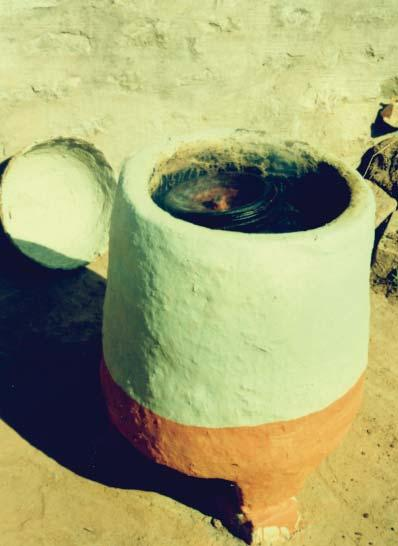
\includegraphics[scale=.31]{images/chap02-24.jpg}
\caption{An earthen oven in a Hindu Gujjar’s house at Mirpur Kotala.}\label{chap02-fig24}
\end{figure}

Generally, the Hindu Gujjar dwelling unit consists of a large living room with an entrance door from the fronting veranda and windows on the sides and back walls. These have regular shutters. The windows are even grilled for safety against wild predators. In front of the room is a spacious veranda, enclosed from the sides, but with an open front. The veranda has been partitioned to make a kitchen on one side, wherein an earthen hearth with multiple cooking-stands is made in a corner. While food may be cooked on the main stand, it is kept warm on the secondary ones. The plinth of the hut is kept about half a metre higher from the surrounding ground. The hut is covered with the usual thatched roof (chhappar). On one side of the hut, a detached jungle wood enclosure is made, to serve as a bathroom. In front of the hut is a well-trimmed earthen courtyard on the ground level. A corner of this courtyard also serves as an open-air kitchen during fair-weather conditions. A neatly made earthen oven with multipurpose cooking-stands may be seen at the corner of this courtyard. One such stand is exclusively reserved for boiling milk in a large earthen pot on the simmering heat of dried cow dung cakes. On that heat, milk never boils to overflow, but it becomes thick, brownish and saturated with the mild aroma of the earthenware. The author can never forget the rich taste of kahadi that he relished in a Gujjar house in this village. Having been prepared in an earthen pot on the simmering heat of cow-dung cakes continuously for 24 hours, that dish was kahadi (a dish cooked and boiled for a prolonged period) in the real sense. On one side of the dwelling is a small kitchen garden and a little away, an improvised but sturdy jungle wood enclosure to tether cows and buffaloes. The homestead is fenced with jungle wood, reeds, and so on, on all sides, to ward off wild predators.

The exterior and interior of the hut is occasionally plastered with mud and cow dung gara and whitewashed. On the whitewashed walls, the women make interesting geometrical, floral, faunal and figural motifs. The doors and windows are framed with colourful bands and floral designs. The Gujjar women are dextrous in making earthenware of great variety and sizes for their daily use. By using bamboo strips and reeds as reinforcement, they prepare large sized boxes and silos for storing household items and grains. These containers (Figure 2.25) are known variously as the kutthala, paichhi, kothi, pedu, and so on. They also make different types of artistic and functional earthen ovens for cooking, boiling milk, heating water, keeping food warm, and so on. Mostly dried cakes made of the dung of buffaloes or cows are used in these ovens. Some of these ovens are even portable and can be conveniently carried from one place to the other (Figure 2.24).

\begin{figure}[!htbp]
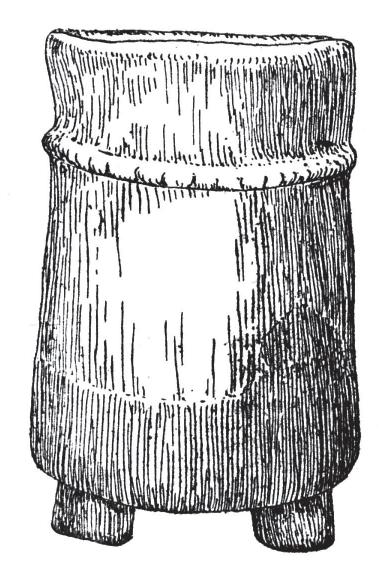
\includegraphics[scale=.35]{images/chap02-25.jpg}
\caption{An earthen kutthala}\label{chap02-fig25}
\end{figure}

For the Hindu Gujjar women, smearing the floors and the front courtyard with cow-dung is a part of their morning routine. While smearing, they create a soothing chiaroscuro effect by the dextrous manipulation of their hands and fingers. They also decorate the earthenware with innumerable stylised geometrical, phyllomorphic, zoomorphic and anthropomorphic devices. At times, they also make these devices in bas-relief and decorate them with locally available earthen pigments and ultramarine blue. These simple creations, bold and crude as these are, impart colour and charm to their humble forest-dwellings (Figures 2.26 and 2.27).

\begin{figure}[!htbp]
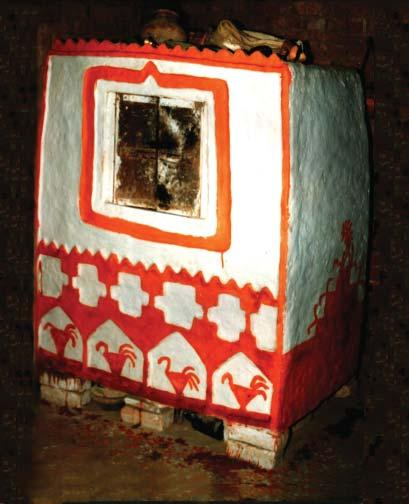
\includegraphics[scale=.34]{images/chap02-26.jpg}
\caption{Decorative work on an earthen silo}\label{chap02-fig26}
\end{figure}


\begin{figure}[H]
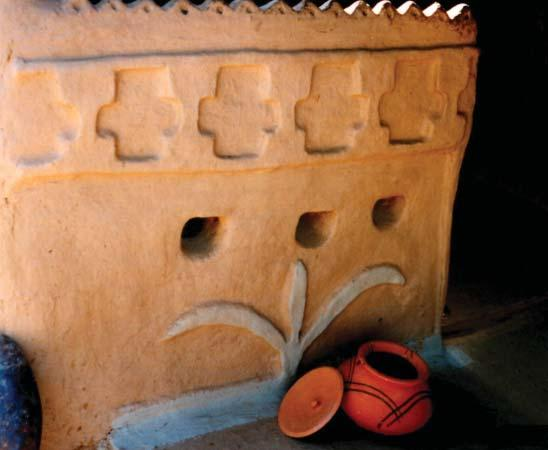
\includegraphics[scale=.34]{images/chap02-27.jpg}
\caption{Bas-relief decoration on an earthen bin}\label{chap02-fig27}
\end{figure}


